\documentclass[aspectratio=169,unknownkeysallowed,xcolor=dvipsnames,beamer]{beamer} %handout,notes=show

\usepackage{textcomp}
\usepackage[utf8]{inputenc}
% Locate graphics where you want
\usepackage[absolute,overlay]{textpos}
% \usepackage{default}
\usepackage{graphicx}
%  \usepackage[pdftex]{hyperref}
\usepackage{url}
\usepackage{amsmath}

% frames have to be fragile
\newif\ifnotes
% \notestrue

%\notestrue


\ifnotes
%\setbeamertemplate{note page}[plain]
\setbeamertemplate{note page}[compress]
\setbeamerfont{note page}{size=\large}
\setbeameroption{show only notes}
%\setbeameroption{show notes}
\usepackage{pgfpages}
\pgfpagesuselayout{2 on 1}[a4paper,border shrink=5mm]%
\else
%\setbeameroption{hide notes}
\fi
%\notesfalse



% nastaveni TypeWriter
%\usepackage{courier}
%\usepackage{lmodern}
%\renewcommand*\ttdefault{txtt}
\DeclareFontShape{OT1}{cmtt}{bx}{n}{<5><6><7><8><9><10><10.95><12><14.4><17.28><20.74><24.88>cmttb10}{}


% \usepackage{verbatim}
\usepackage[absolute,overlay]{textpos}

\usepackage{listings}
% \usepackage{courier}
\definecolor{grey}{RGB}{70,70,70}
\definecolor{green}{RGB}{0,255,0}
\definecolor{red}{RGB}{202,53,53}
\definecolor{lightGrey}{RGB}{250,250,250}
\definecolor{darkGrey}{RGB}{50,50,50}


\usepackage{color}
\definecolor{lightgray}{rgb}{.9,.9,.9}
\definecolor{darkgray}{rgb}{.4,.4,.4}
\definecolor{purple}{rgb}{0.65, 0.12, 0.82}

 \usetheme{Boadilla}
% \usetheme{Berkeley}
%\usetheme{Goettingen}
% \usetheme{Montpellier}
% \usetheme{Warsaw}
% \usetheme{Madrid}
% \usetheme{Szeged}
% \useoutertheme{infolines}
%\usecolortheme[named=MidnightBlue]{structure}
\usecolortheme[named=OliveGreen]{structure}
%\usecolortheme[named=PineGreen]{structure}
% \setbeamertemplate{navigation symbols}{}


\title[FOSS4G - OSHW]
{Lake thermodynamic fluxes monitoring with OSHW and FOSS4G}
%\subtitle{SVO\v{C}}
%\pdforstring{}{}
\author{Yann Chemin}
\date{\tiny October 22th, 2016}


%\AtBeginSection[]{\begin{frame}\frametitle{Obsah}%
%\tableofcontents[currentsection ]\end{frame}}
%\AtBeginSubsection[]
%{
%  \begin{frame}<beamer>
%  \frametitle{Obsah}
%  \tableofcontents[currentsection,currentsubsection]
%  \end{frame}
%}

\setbeamercovered{transparent}

\hypersetup{%
	pdfauthor={Yann Chemin},%
	pdfsubject={Presentation},%
    pdfkeywords={FOSS4G, OSHW, RaspberryPI, ET, Raingauge, OSGEO}
}

\usepackage{listings}
\lstdefinestyle{C++}{%
  % language
  language=C++, % [ANSI]C++, GNU, ISO, Visual
  basicstyle=\ttfamily\small,
  commentstyle=\itshape,
  keywordstyle=\bfseries, % needs another \ttdefault
  showstringspaces=false,
  stringstyle=,
  identifierstyle=,
  % working with latex
  escapeinside={//lst}{\^^M}  
}

\lstset{%
%  frame=trBL,
%  backgroundcolor=\color{},
  linewidth=\textwidth,
  % working with latex
  gobble=2,
  % float
  nolol=false,
  numberbychapter=true,
  captionpos=t,% tb
  % breaking lines
  breaklines=true,
  breakatwhitespace=true,
  breakindent=10em,
  breakautoindent=true,
  prebreak={},
  postbreak={},
  %document default style
    basicstyle=\ttfamily
}


%\lstlistlistingname % The header name for the list of listings.
%\lstlistingname % The caption label for listings.

\lstnewenvironment{cmdline}[1][]
{\lstset{
  style=C++,
  #1}}
{}

\lstnewenvironment{scpp}[1][]
{\lstset{
  style=C++,
  #1}}
{}

\lstnewenvironment{ncpp}[1][]
{\lstset{
  style=C++,
  numbers=left, 
  numberstyle=\scriptsize, 
  stepnumber=1,
  numbersep=5pt,
  #1}}
{}

\lstnewenvironment{fcpp}[1][]
{\lstset{
  style=C++,
  float,
   % line numbers
  numbers=left, 
  numberstyle=\scriptsize, 
  stepnumber=1,
  numbersep=5pt,
  #1}}
{}


\lstnewenvironment{lcpp}[1][]
{\lstset{%
style=C++,
numbers=left, 
numberstyle=\scriptsize, 
stepnumber=1,
numbersep=5pt,
xleftmargin=12pt,
breakautoindent=false,
breaklines=false,%
#1}}{}

\lstnewenvironment{smallcpp}[1][]
{\lstset{%
style=C++,
numbers=left, 
numberstyle=\tiny, 
stepnumber=1,
numbersep=5pt,
xleftmargin=12pt,
breakautoindent=false,
breaklines=false,%
basicstyle=\ttfamily\scriptsize,
#1}}{}


\lstnewenvironment{pscpp}[1][]
{\lstset{%
style=C++,
xleftmargin=12pt,
breakautoindent=false,
breaklines=false,
#1}}{}


%\lstset{index={square},index={[2]root}}


\newcommand{\overovaciref}[1]{{\scriptsize(\ref{#1})}}


\usepackage{tipa}
\newcommand{\pron}[2]{#1 [#2]}

%%%%%%%%%%%%%%%%%%%%%%%%%%%%%%%%%%%%%%%%%%%%%%%%%%%%%%%%%%%%%%%%%%%%
% TOC frame setup
%%%%%%%%%%%%%%%%%%%%%%%%%%%%%%%%%%%%%%%%%%%%%%%%%%%%%%%%%%%%%%%%%%%%
\usepackage{multicol}
\colorlet{mycolor}{orange!80!black}% change this color to suit your needs
\AtBeginSection[]{
  \setbeamercolor{section in toc shaded}{use=structure,fg=structure.fg}
  \setbeamercolor{section in toc}{fg=mycolor}
  \setbeamercolor{subsection in toc shaded}{fg=black}
  \setbeamercolor{subsection in toc}{fg=mycolor}
  \frame<beamer>{\begin{multicols}{2}
  \frametitle{Outline}
  \setcounter{tocdepth}{2}  
  \tableofcontents[currentsection,subsections]
\end{multicols} 
 }
}

\setbeamercolor{author in head/foot}{fg=white}
\setbeamercolor{title in head/foot}{fg=white}
\setbeamercolor{section in head/foot}{fg=mycolor}
\setbeamertemplate{section in head/foot shaded}{\color{white!70!black}\insertsectionhead}
\setbeamercolor{subsection in head/foot}{fg=mycolor}
\setbeamertemplate{subsection in head/foot shaded}{\color{white!70!black}\insertsubsectionhead}
\setbeamercolor{frametitle}{fg=white}
\setbeamercolor{framesubtitle}{fg=white}

%%%%%%%%%%%%%%%%%%%%%%%%%%%%%%%%%%%%%%%%%%%%%%%%%%%%%%%%%%%%%%%%%%%%
%%%%%%%%%%%%%%%%%%%%%%%%%%%%%%%%%%%%%%%%%%%%%%%%%%%%%%%%%%%%%%%%%%%%
%%%%%%%%%%%%%%%%%%%%%%%%%%%%%%%%%%%%%%%%%%%%%%%%%%%%%%%%%%%%%%%%%%%%
\begin{document}


%%%%%%%%%%%%%%%%%%%%%%%%%%%%%%%%%%%%%%%%%%%%%%%%%%%%%%%%%%%%%%%%%%%%
\begin{frame}
\begin{center}
 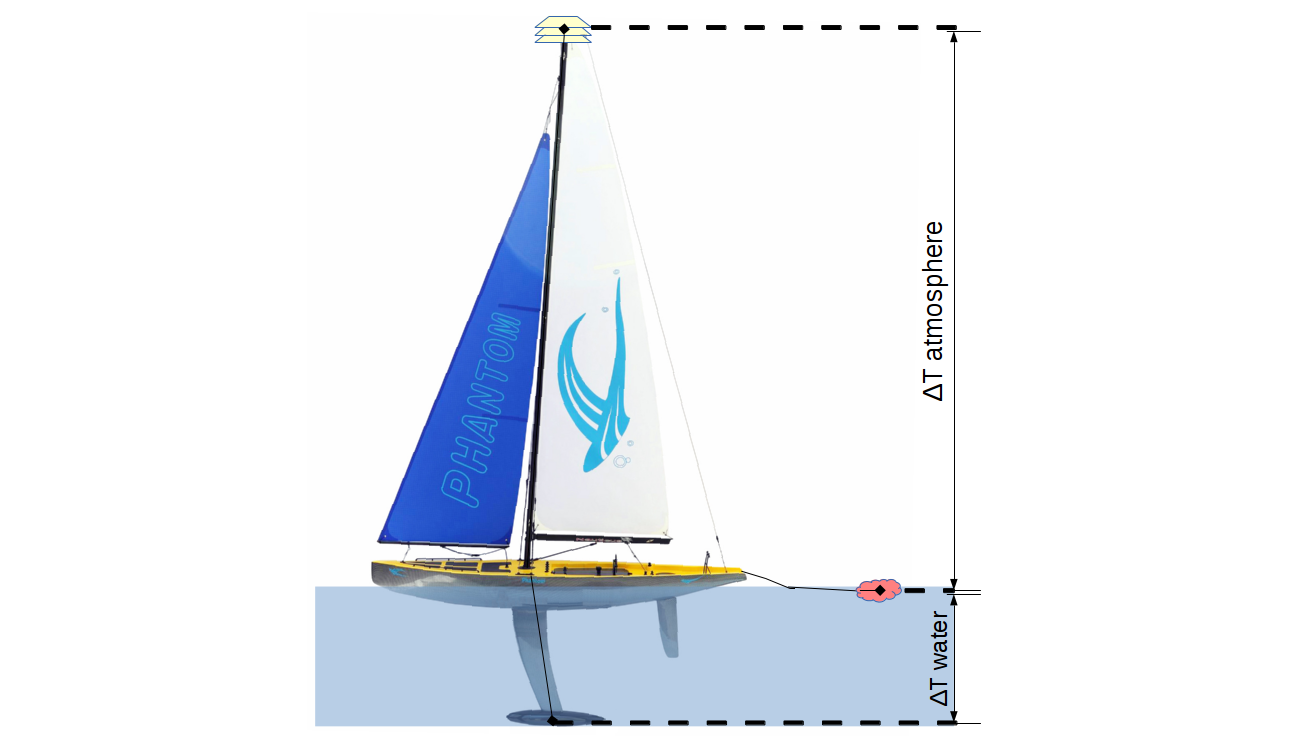
\includegraphics[width=5cm]{amitomiv1}
\end{center}
 \maketitle
 \end{frame}
%%%%%%%%%%%%%%%%%%%%%%%%%%%%%%%%%%%%%%%%%%%%%%%%%%%%%%%%%%%%%%%%%%%%

%%%%%%%%%%%%%%%%%%%%%%%%%%%%%%%%%%%%%%%%%%%%%%%%%%%%%%%%%%%%%%%%%%%%
\begin{frame}{Contents}
 \begin{multicols}{2}
  \setcounter{tocdepth}{2}  
  \tableofcontents
 \end{multicols} 
\end{frame}
%%%%%%%%%%%%%%%%%%%%%%%%%%%%%%%%%%%%%%%%%%%%%%%%%%%%%%%%%%%%%%%%%%%%

\section{Introduction}
\subsection{Scientific Issue}
%%%%%%%%%%%%%%%%%%%%%%%%%%%%%%%%%%%%%%%%%%%%%%%%%%%%%%%%%%%%%%%%%%%%
\begin{frame}[fragile]{Overview}
\textbf{The Scientific Problem:}
\newline\linebreak
\textbf{\textcolor{brown}{Monitoring Evapotranspiration from Space for Water Management}}
\newline\linebreak 
\begin{itemize}
 \item ET = E+T
 \item Evaporation + Transpiration
 \item Evapotranspiration calibration \& modeling
 \item Lakes of various sizes
 \item controlled, ungauged
 \item Rural tanks in Asia
\end{itemize}
\end{frame}

\subsection{Agricultural water equity}
%%%%%%%%%%%%%%%%%%%%%%%%%%%%%%%%%%%%%%%%%%%%%%%%%%%%%%%%%%%%%%%%%%%%
\begin{frame}[fragile]{Equity of water use in irrigation systems}

\textbf{Irrigation water monitoring \& management}
\begin{itemize}
 \item Map: Uniform colour is equity of water distribution
 \item Graph: Irrigation system equity (mm/d, daily, 12 years)
\end{itemize}

\begin{columns}
\column{0.4\textwidth}
\begin{center}
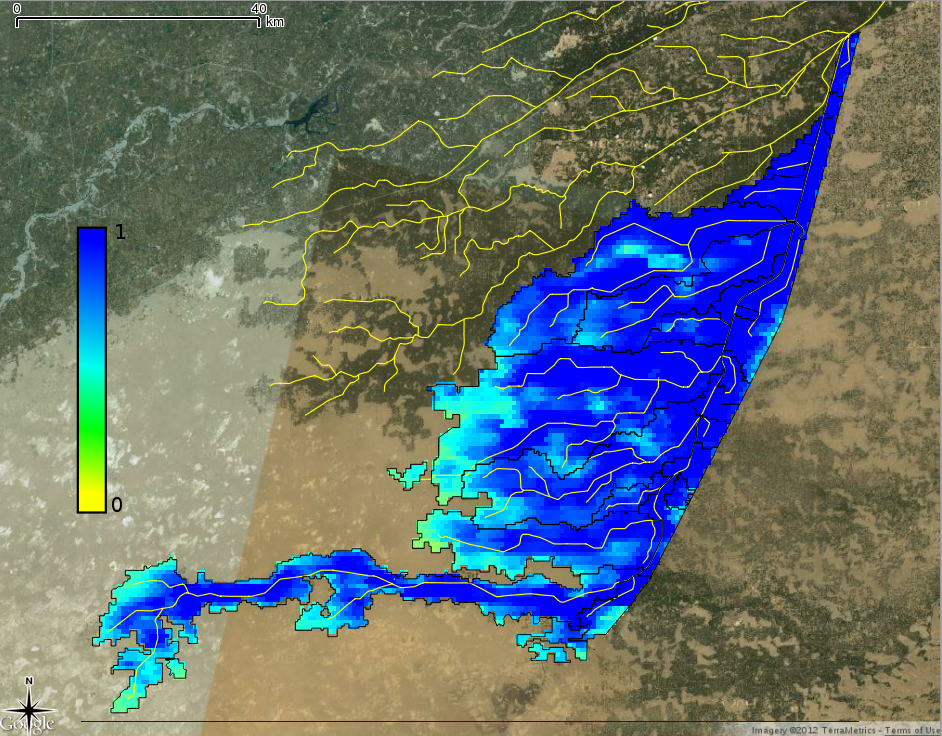
\includegraphics[width=5cm]{fess2012ef}
\end{center}

\column{0.6\textwidth}
\begin{flushleft}
  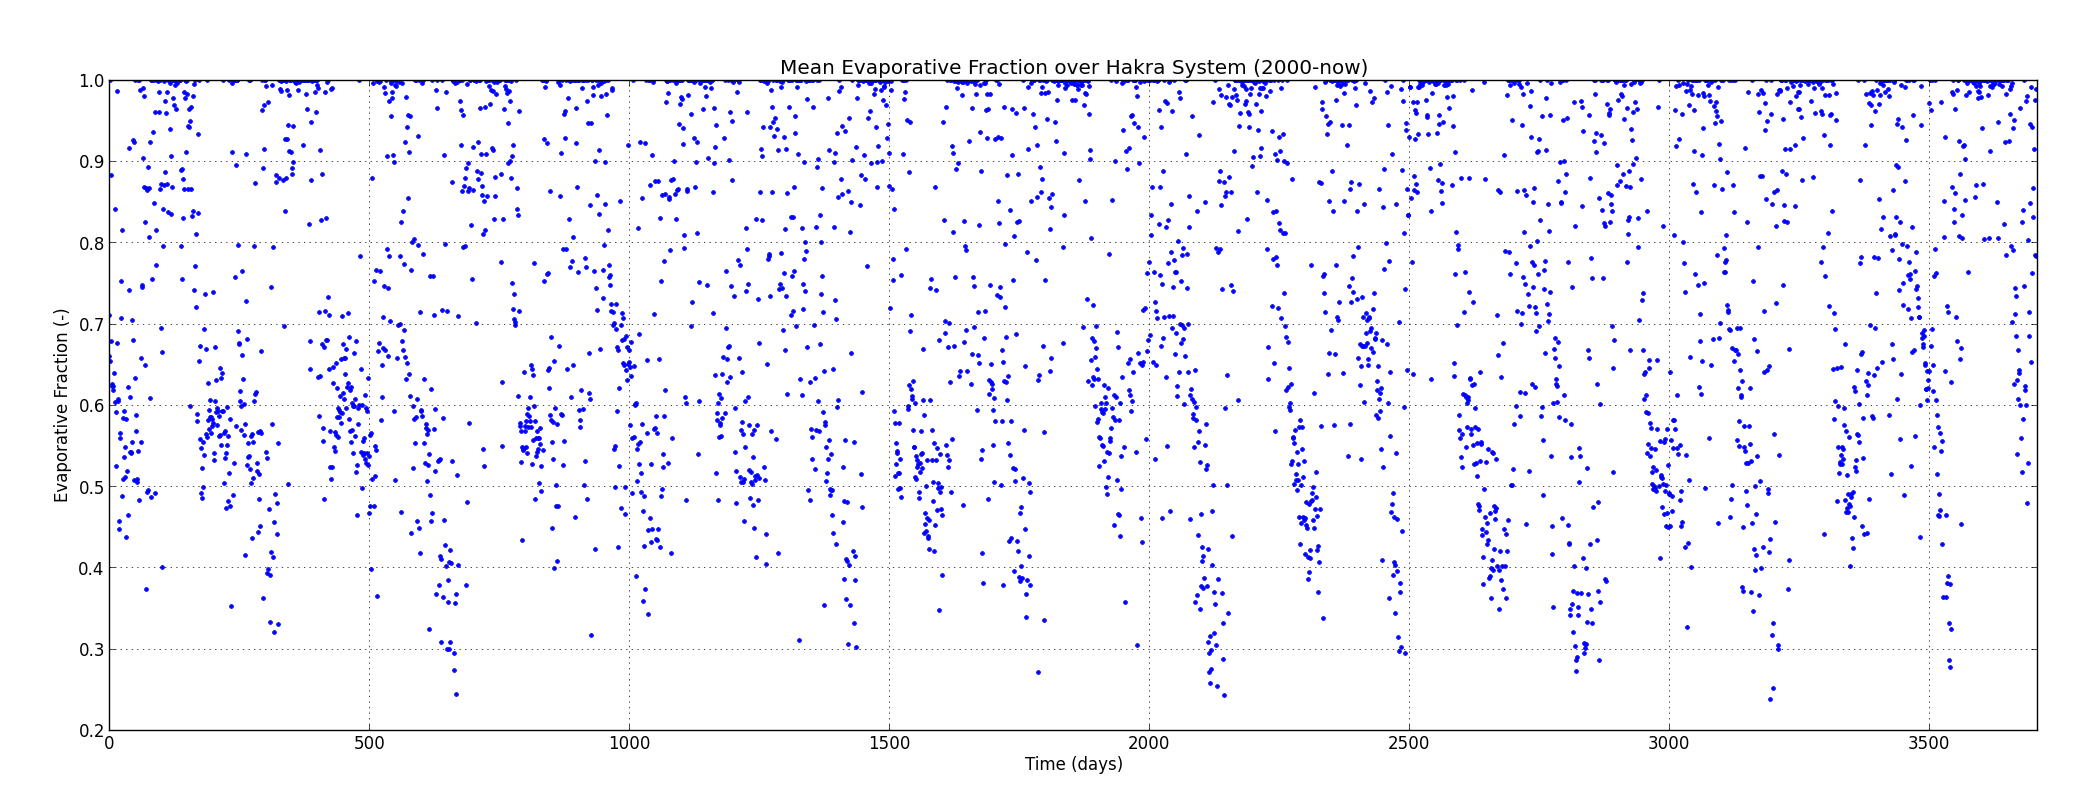
\includegraphics[width=9cm]{fess2012meaneftemporal}
\end{flushleft}
\end{columns}
% Evaporative Fraction 2012 October 4th Hakra, Punjab, Pakistan ~4000 images (2000-2012)
\end{frame}

\subsection{Country water monitoring}
%%%%%%%%%%%%%%%%%%%%%%%%%%%%%%%%%%%%%%%%%%%%%%%%%%%%%%%%%%%%%%%%%%%%
{\usebackgroundtemplate{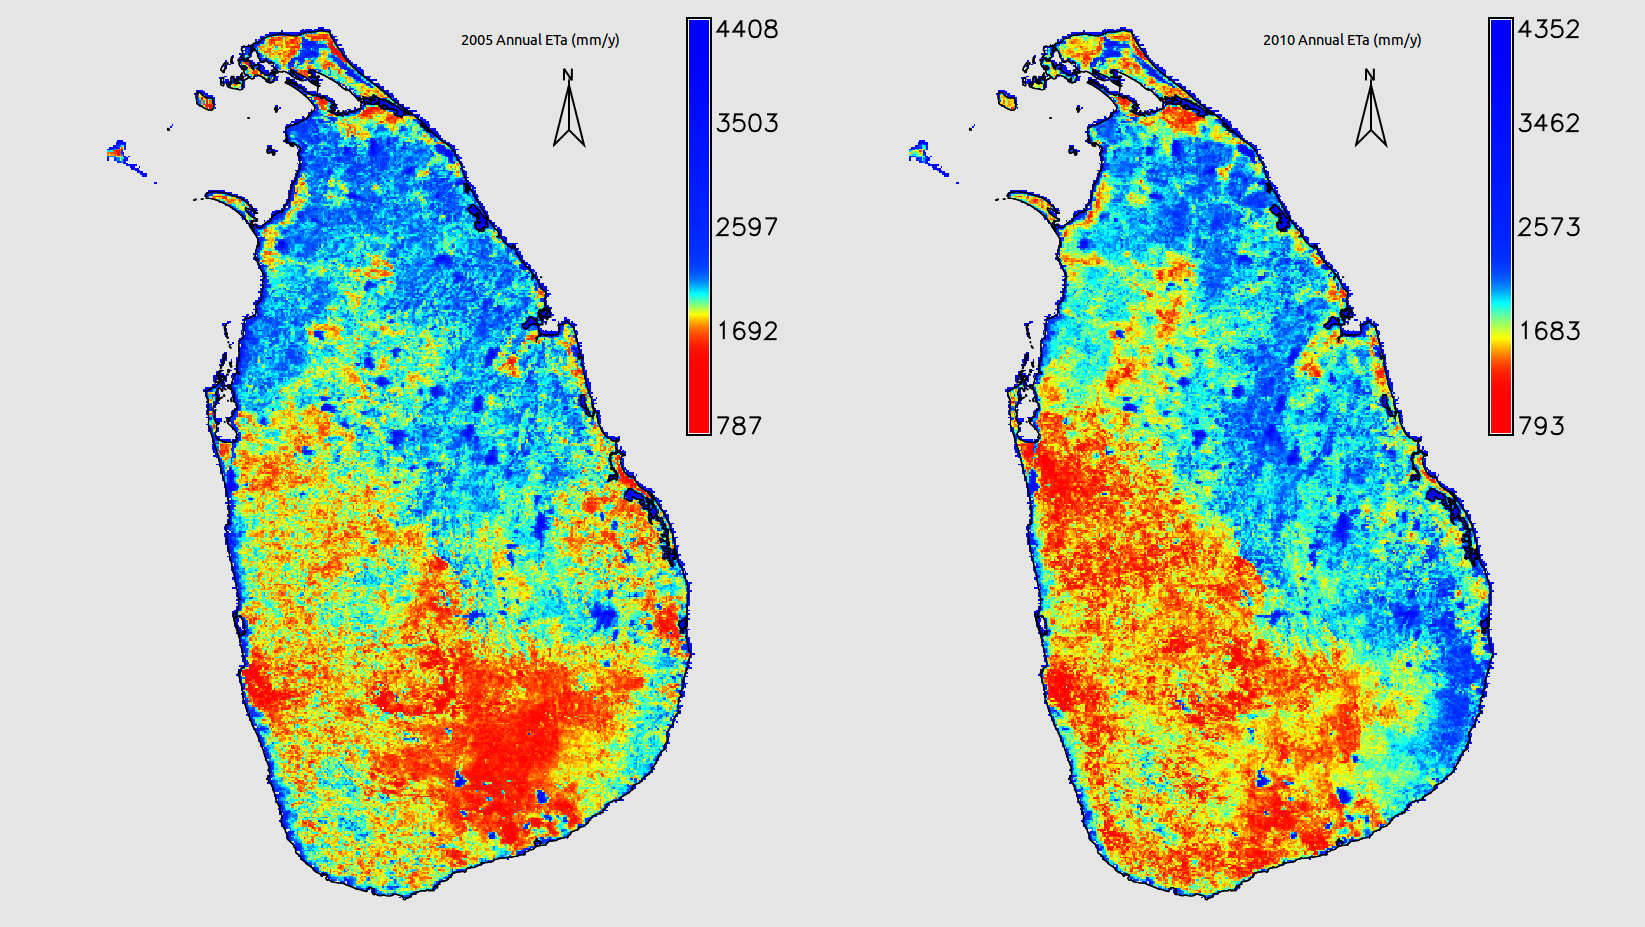
\includegraphics[height=\paperheight,width=\paperwidth]{slet2005_2010}}
\begin{frame}[plain]
\end{frame}}

\subsection{ET Models Benchmarking}
%%%%%%%%%%%%%%%%%%%%%%%%%%%%%%%%%%%%%%%%%%%%%%%%%%%%%%%%%%%%%%%%%%%%
\begin{frame}[fragile]{ET models Benchmarking}

\begin{center}
 Average ET for Sri Lanka, Daily 2000-2012 (mm/d, daily, 12.3 years)
 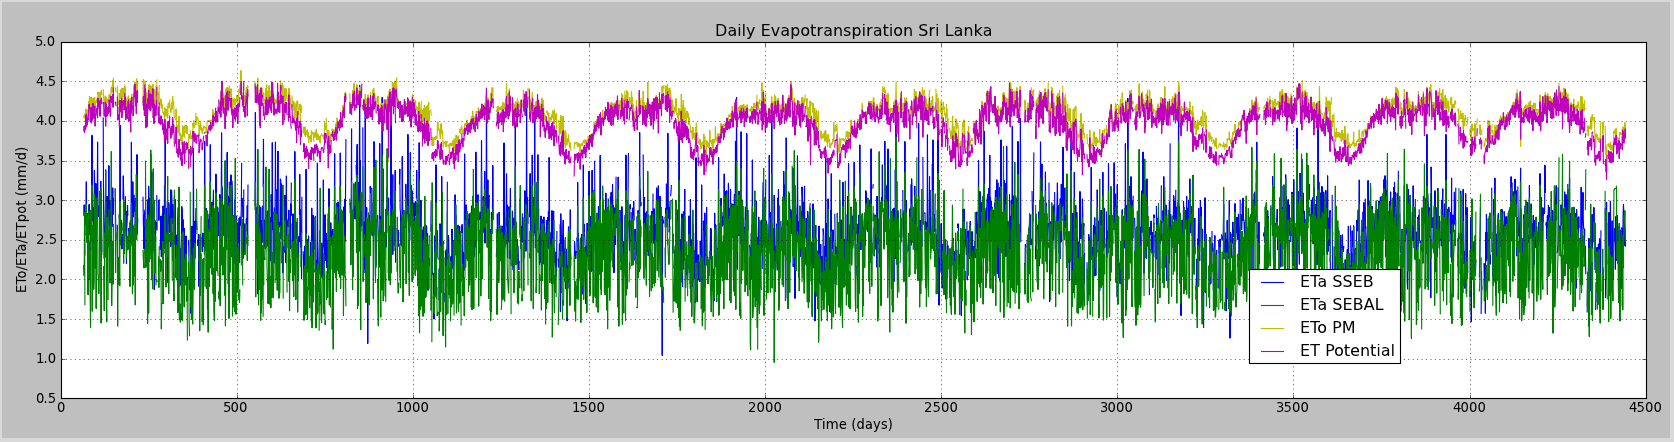
\includegraphics[width=15cm]{sltemporaletb}
\end{center}

\begin{block}{Comparison}
\begin{itemize}
 \item ETo \& ETpot (rad) are similar, expected.
 \item ETa models are not so similar, expected.
 \item ETo \& ETpot (rad) are higher than ETa models, expected.
\end{itemize}

\end{block}
\end{frame}


\section{Frameworks}
\subsection{Chain processing}
%%%%%%%%%%%%%%%%%%%%%%%%%%%%%%%%%%%%%%%%%%%%%%%%%%%%%%%%%%%%%%%%%%%%
\begin{frame}[fragile]{Chain processing}

\textbf{Chain processing}\\
 has a fundamental impact on remote sensing work:\newline\linebreak

\begin{itemize}
 \item Standardization limits bugs
 \item Less prone to human error
 \item Simpler parameterization access
 \item Permits to apply any number of modules to all target images
 \item Ensures maximum quality of generated images
\end{itemize}
\end{frame}

\subsection{Blueprint}
%%%%%%%%%%%%%%%%%%%%%%%%%%%%%%%%%%%%%%%%%%%%%%%%%%%%%%%%%%%%%%%%%%%%
\begin{frame}[fragile]{Blueprint}

\begin{center}
 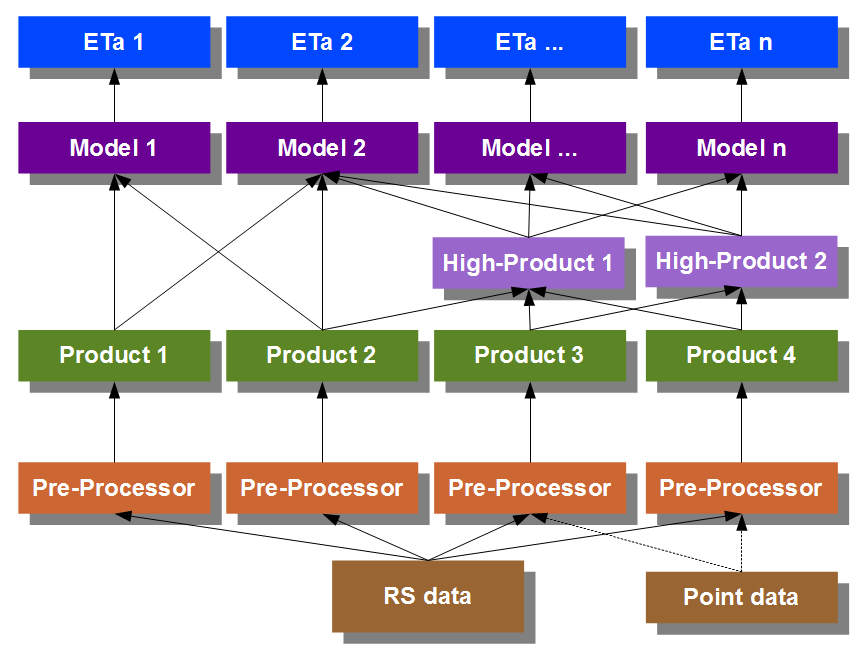
\includegraphics[width=7.5cm]{chain0}
\end{center}

\begin{itemize}
 \item GDAL+[C+OpenMP]
 \item GRASSGIS+pyGRASS+[C+OpenMP]
\end{itemize}
\end{frame}

\subsection{GDAL}
%%%%%%%%%%%%%%%%%%%%%%%%%%%%%%%%%%%%%%%%%%%%%%%%%%%%%%%%%%%%%%%%%%%%
\begin{frame}[fragile]{GDAL framework}
\frametitle{ GDAL+[C+OpenMP]}
\begin{center}
 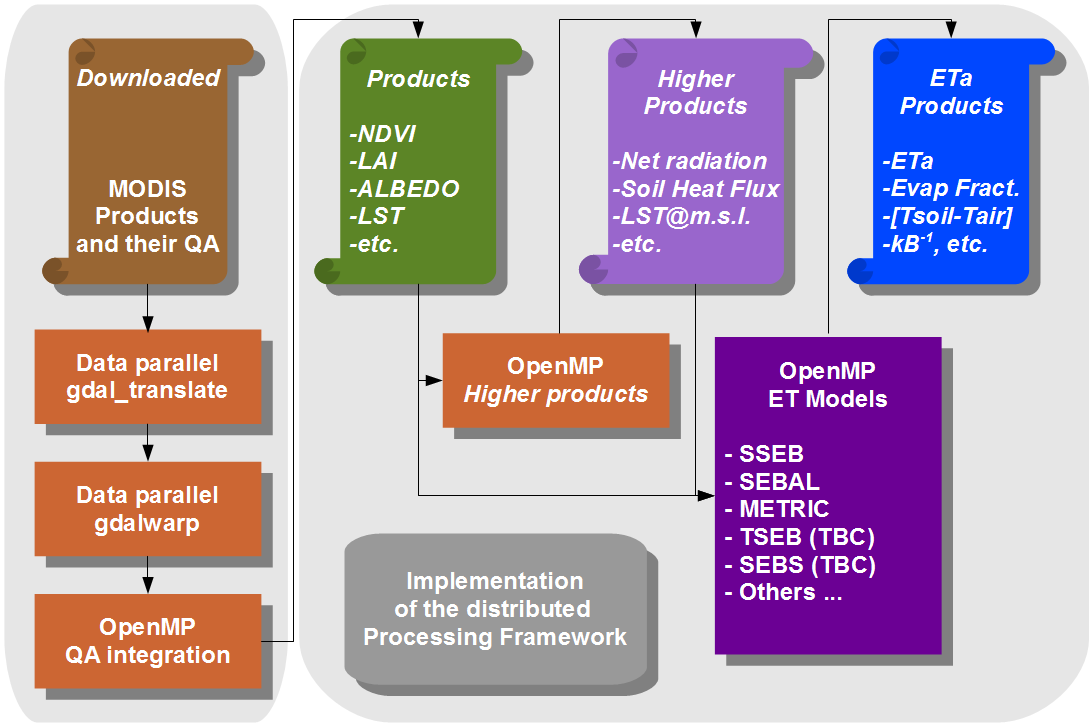
\includegraphics[width=10.5cm]{chain2}
\end{center}
\end{frame}

%%%%%%%%%%%%%%%%%%%%%%%%%%%%%%%%%%%%%%%%%%%%%%%%%%%%%%%%%%%%%%%%%%%%
\begin{frame}[fragile]{GDAL framework}

\begin{columns}
\column[t]{0.6\textwidth}
\begin{center}
 OpenMP Distribution \\
 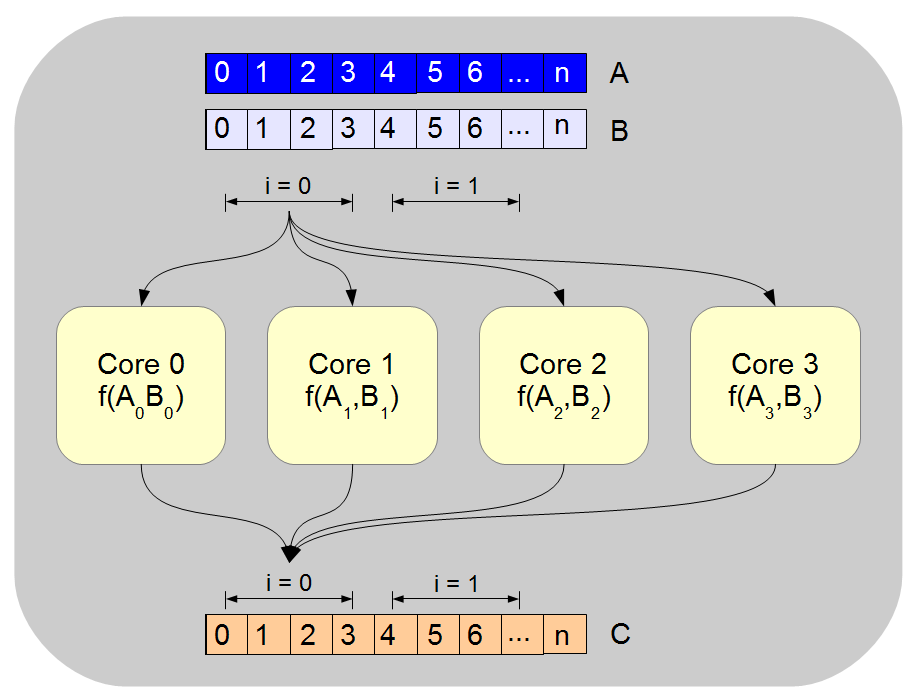
\includegraphics[width=7.5cm]{chain1}
\end{center}
\column[t]{0.4\textwidth}
\begin{center}
 Cores \\
 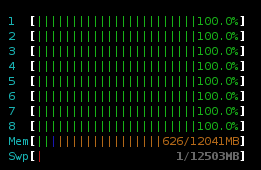
\includegraphics[width=5cm]{cores}
\end{center}
\end{columns}
\end{frame}



\subsection{GRASS GIS big data framework}
%%%%%%%%%%%%%%%%%%%%%%%%%%%%%%%%%%%%%%%%%%%%%%%%%%%%%%%%%%%%%%%%%%%%
\begin{frame}[fragile]{GRASS GIS framework}

\begin{center}
 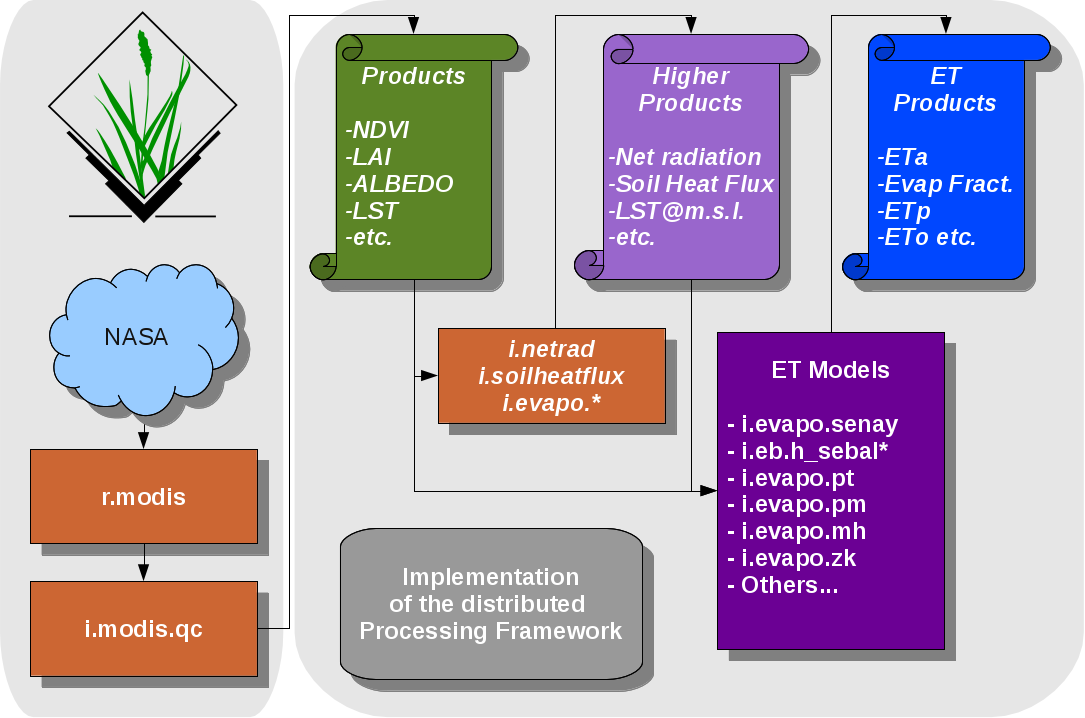
\includegraphics[width=8.5cm]{architecture_implementation}
\end{center}

\end{frame}

\subsection{metaModule}
%%%%%%%%%%%%%%%%%%%%%%%%%%%%%%%%%%%%%%%%%%%%%%%%%%%%%%%%%%%%%%%%%%%%
\begin{frame}[fragile]{metaModule Concept}

Pythonizing GRASS:\\ From Shell commands to Python functions 

\begin{block}{metaModule concept}
\begin{enumerate}
 \item {\bf GRASS GIS:} Specific image processing modules
 \item {\bf PyWPS:} GRASS modules called by Python
 \item {\bf GRASS script:} GRASS modules called by Python: metaModule
 \item {\bf pyGRASS:} GRASS modules called as Python function: metaModule
 \item {\bf PyWPS v4:} pyGRASS metaModule used directly
\end{enumerate}

\end{block}

\end{frame}

\subsection{pyGRASS}
%%%%%%%%%%%%%%%%%%%%%%%%%%%%%%%%%%%%%%%%%%%%%%%%%%%%%%%%%%%%%%%%%%%%
\begin{frame}[fragile]{pyGRASS metaModule}

\begin{center}
 Summary for Landsat pyGRASS metaModule
 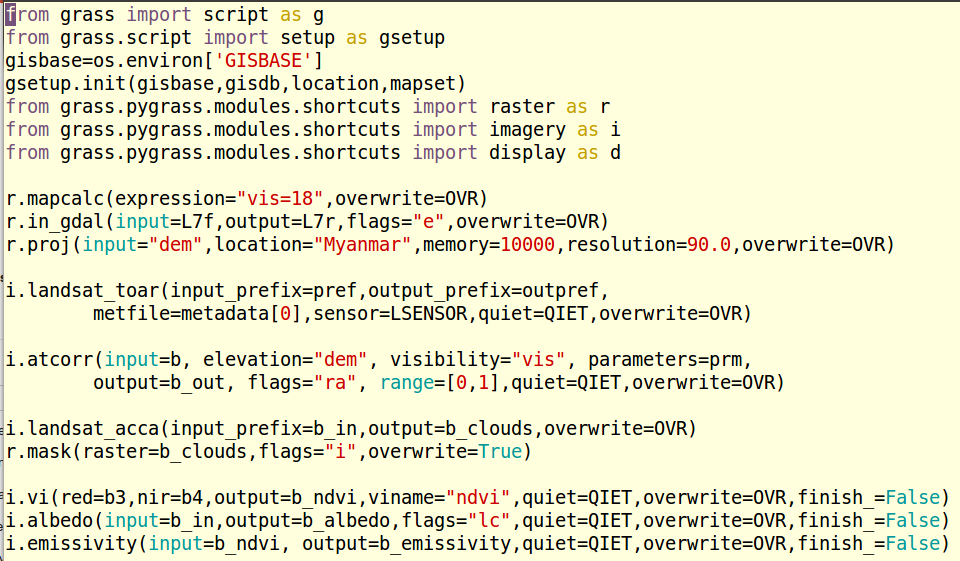
\includegraphics[width=10cm]{pyGRASS1}\\
 \href{http://grasswiki.osgeo.org/wiki/Python/pygrass}{http://grasswiki.osgeo.org/wiki/Python/pygrass}
\end{center}

\end{frame}

\subsection{PyWPS}
%%%%%%%%%%%%%%%%%%%%%%%%%%%%%%%%%%%%%%%%%%%%%%%%%%%%%%%%%%%%%%%%%%%%
\begin{frame}[fragile]{PyWPS}
 Developed by Jachym Cepicky (\href{http://les-ejk.cz/}{http://les-ejk.cz/})
\begin{columns}
\column{0.7\textwidth}
 \begin{itemize}
  \item OGC WPS standard
  \item Server side
  \item Written in Python Language
  \item Version 4 in the making
  \item v4 Low-level API: integration with GRASS GIS
  \item v4 Possible pyGRASS support
 \end{itemize}

\column{0.3\textwidth}
\begin{flushright}
  
\includegraphics[width=4cm]{pywps}
\end{flushright}
\end{columns}
\hspace{10mm}
% {\small {\bf from} pywps {\bf import} (Process, Service, WPSResponse, LiteralInput,
%                    ComplexInput, Format, FileReference)}
\end{frame}

%%%%%%%%%%%%%%%%%%%%%%%%%%%%%%%%%%%%%%%%%%%%%%%%%%%%%%%%%%%%%%%%%%%%
\begin{frame}[fragile]{PyWPS system used in FESS study}

\begin{block}{PyWPS v2 style}
\begin{center}
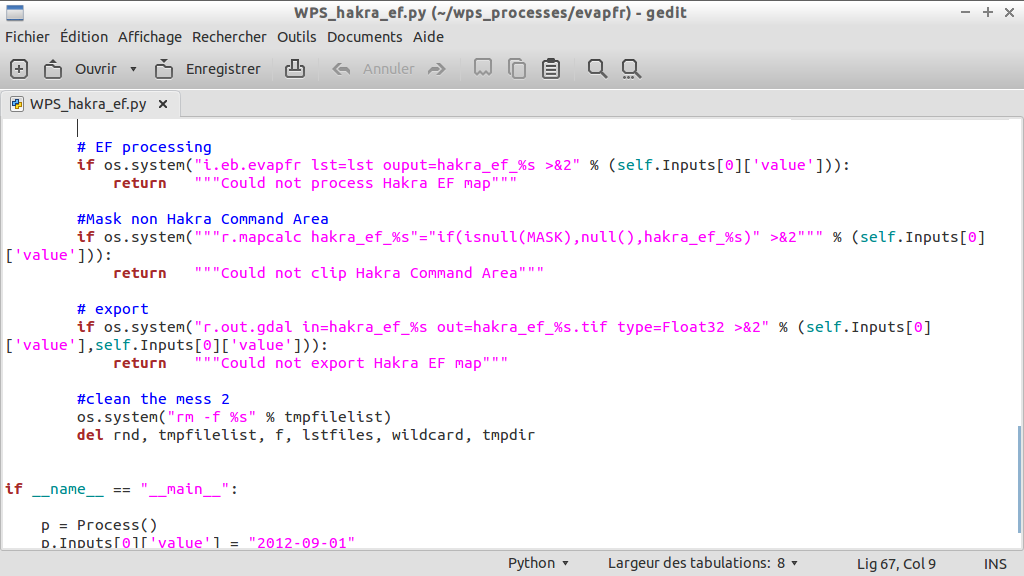
\includegraphics[width=10cm]{pywps_hakra}
\end{center}
\end{block}
\end{frame}


%%%%%%%%%%%%%%%%%%%%%%%%%%%%%%%%%%%%%%%%%%%%%%%%%%%%%%%%%%%%%%%%%%%%
%%%%%%%%%%%%%%%%%%%%%%%%%%%%%%%%%%%%%%%%%%%%%%%%%%%%%%%%%%%%%%%%%%%%
%%%%%%%%%%%%%%%%%%%%%%%%%%%%%%%%%%%%%%%%%%%%%%%%%%%%%%%%%%%%%%%%%%%%



\section{MWS}
\subsection{Rationale for local data}
%%%%%%%%%%%%%%%%%%%%%%%%%%%%%%%%%%%%%%%%%%%%%%%%%%%%%%%%%%%%%%%%%%%%
{\usebackgroundtemplate{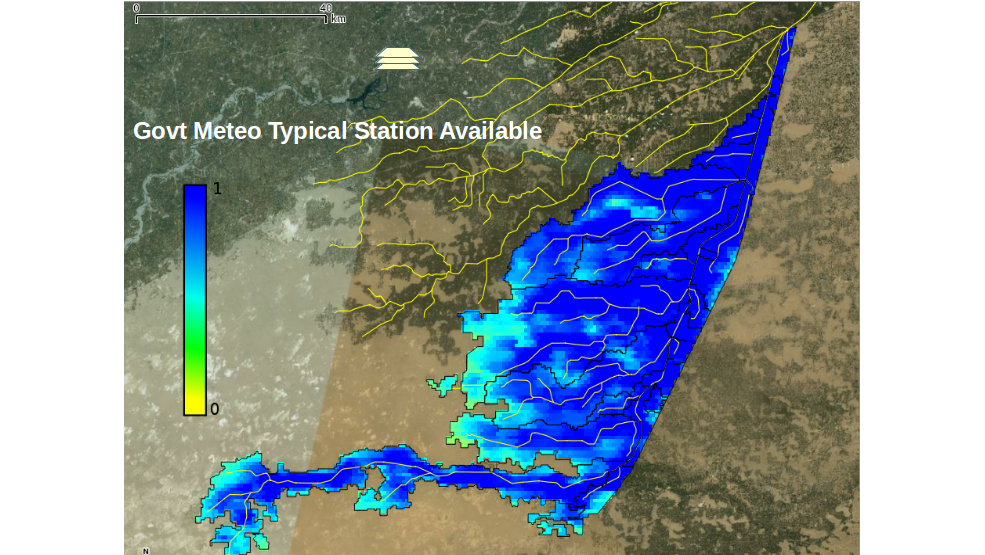
\includegraphics[height=\paperheight,width=\paperwidth]{MWS_v1_deltaT_rationale_0}}
\begin{frame}[plain]
\end{frame}}

%%%%%%%%%%%%%%%%%%%%%%%%%%%%%%%%%%%%%%%%%%%%%%%%%%%%%%%%%%%%%%%%%%%%
{\usebackgroundtemplate{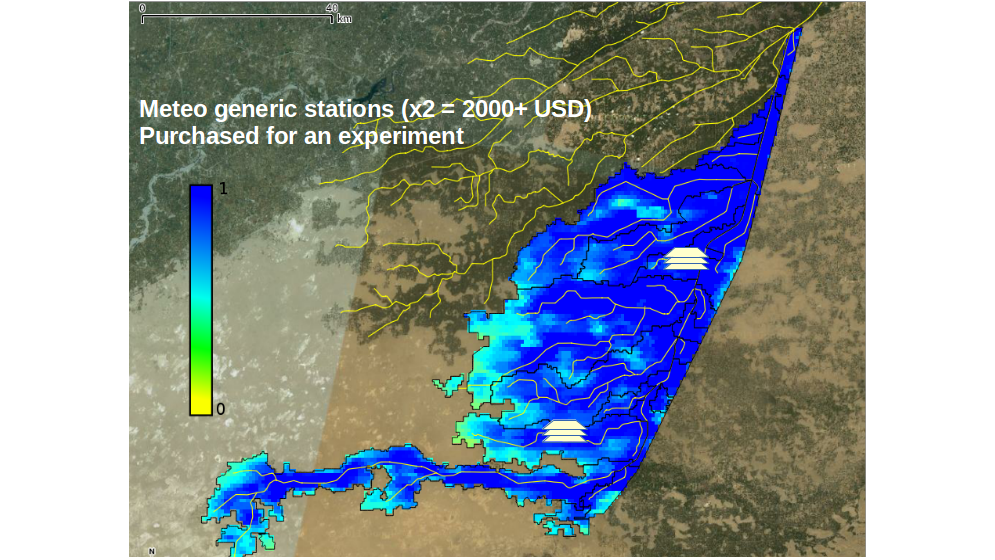
\includegraphics[height=\paperheight,width=\paperwidth]{MWS_v1_deltaT_rationale_1}}
\begin{frame}[plain]
\end{frame}}

%%%%%%%%%%%%%%%%%%%%%%%%%%%%%%%%%%%%%%%%%%%%%%%%%%%%%%%%%%%%%%%%%%%%
{\usebackgroundtemplate{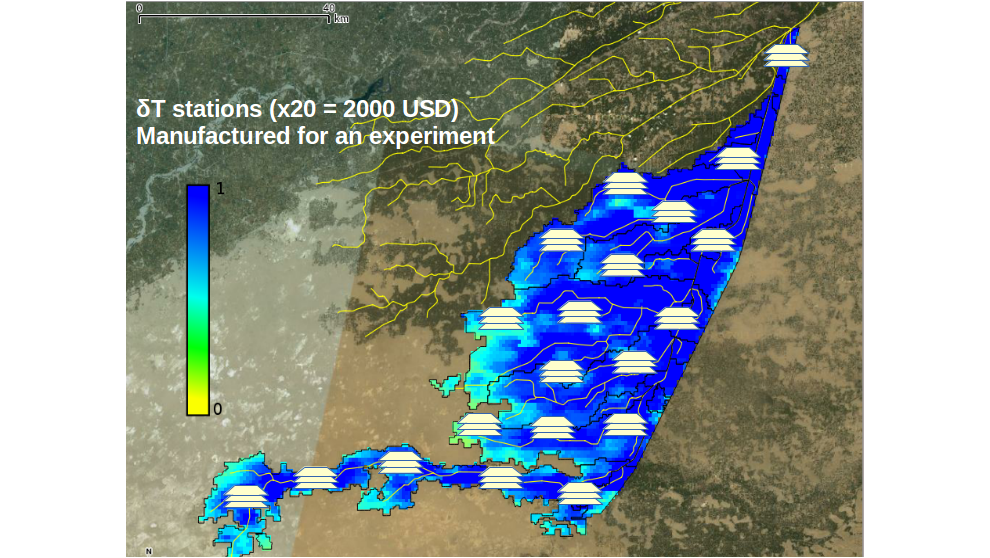
\includegraphics[height=\paperheight,width=\paperwidth]{MWS_v1_deltaT_rationale_2}}
\begin{frame}[plain]
\end{frame}}

\subsection{MWS}
%%%%%%%%%%%%%%%%%%%%%%%%%%%%%%%%%%%%%%%%%%%%%%%%%%%%%%%%%%%%%%%%%%%%
\begin{frame}[fragile]{Open Source Hardware Micro Weather Station v1}

\textbf{Micro Weather Station v1:}\\
Temperature Profiler for ET models calibration
\vspace{5mm}
\begin{itemize}
 \item Arduino Pro 3.3V
 \item Water-proof Digital Temperature Sensors
 \item Li-ion Battery + Solar Panel
 \item OpenLog data logger with SD card
 \item Cost $<$ 100 USD
\end{itemize}
\begin{flushright}
  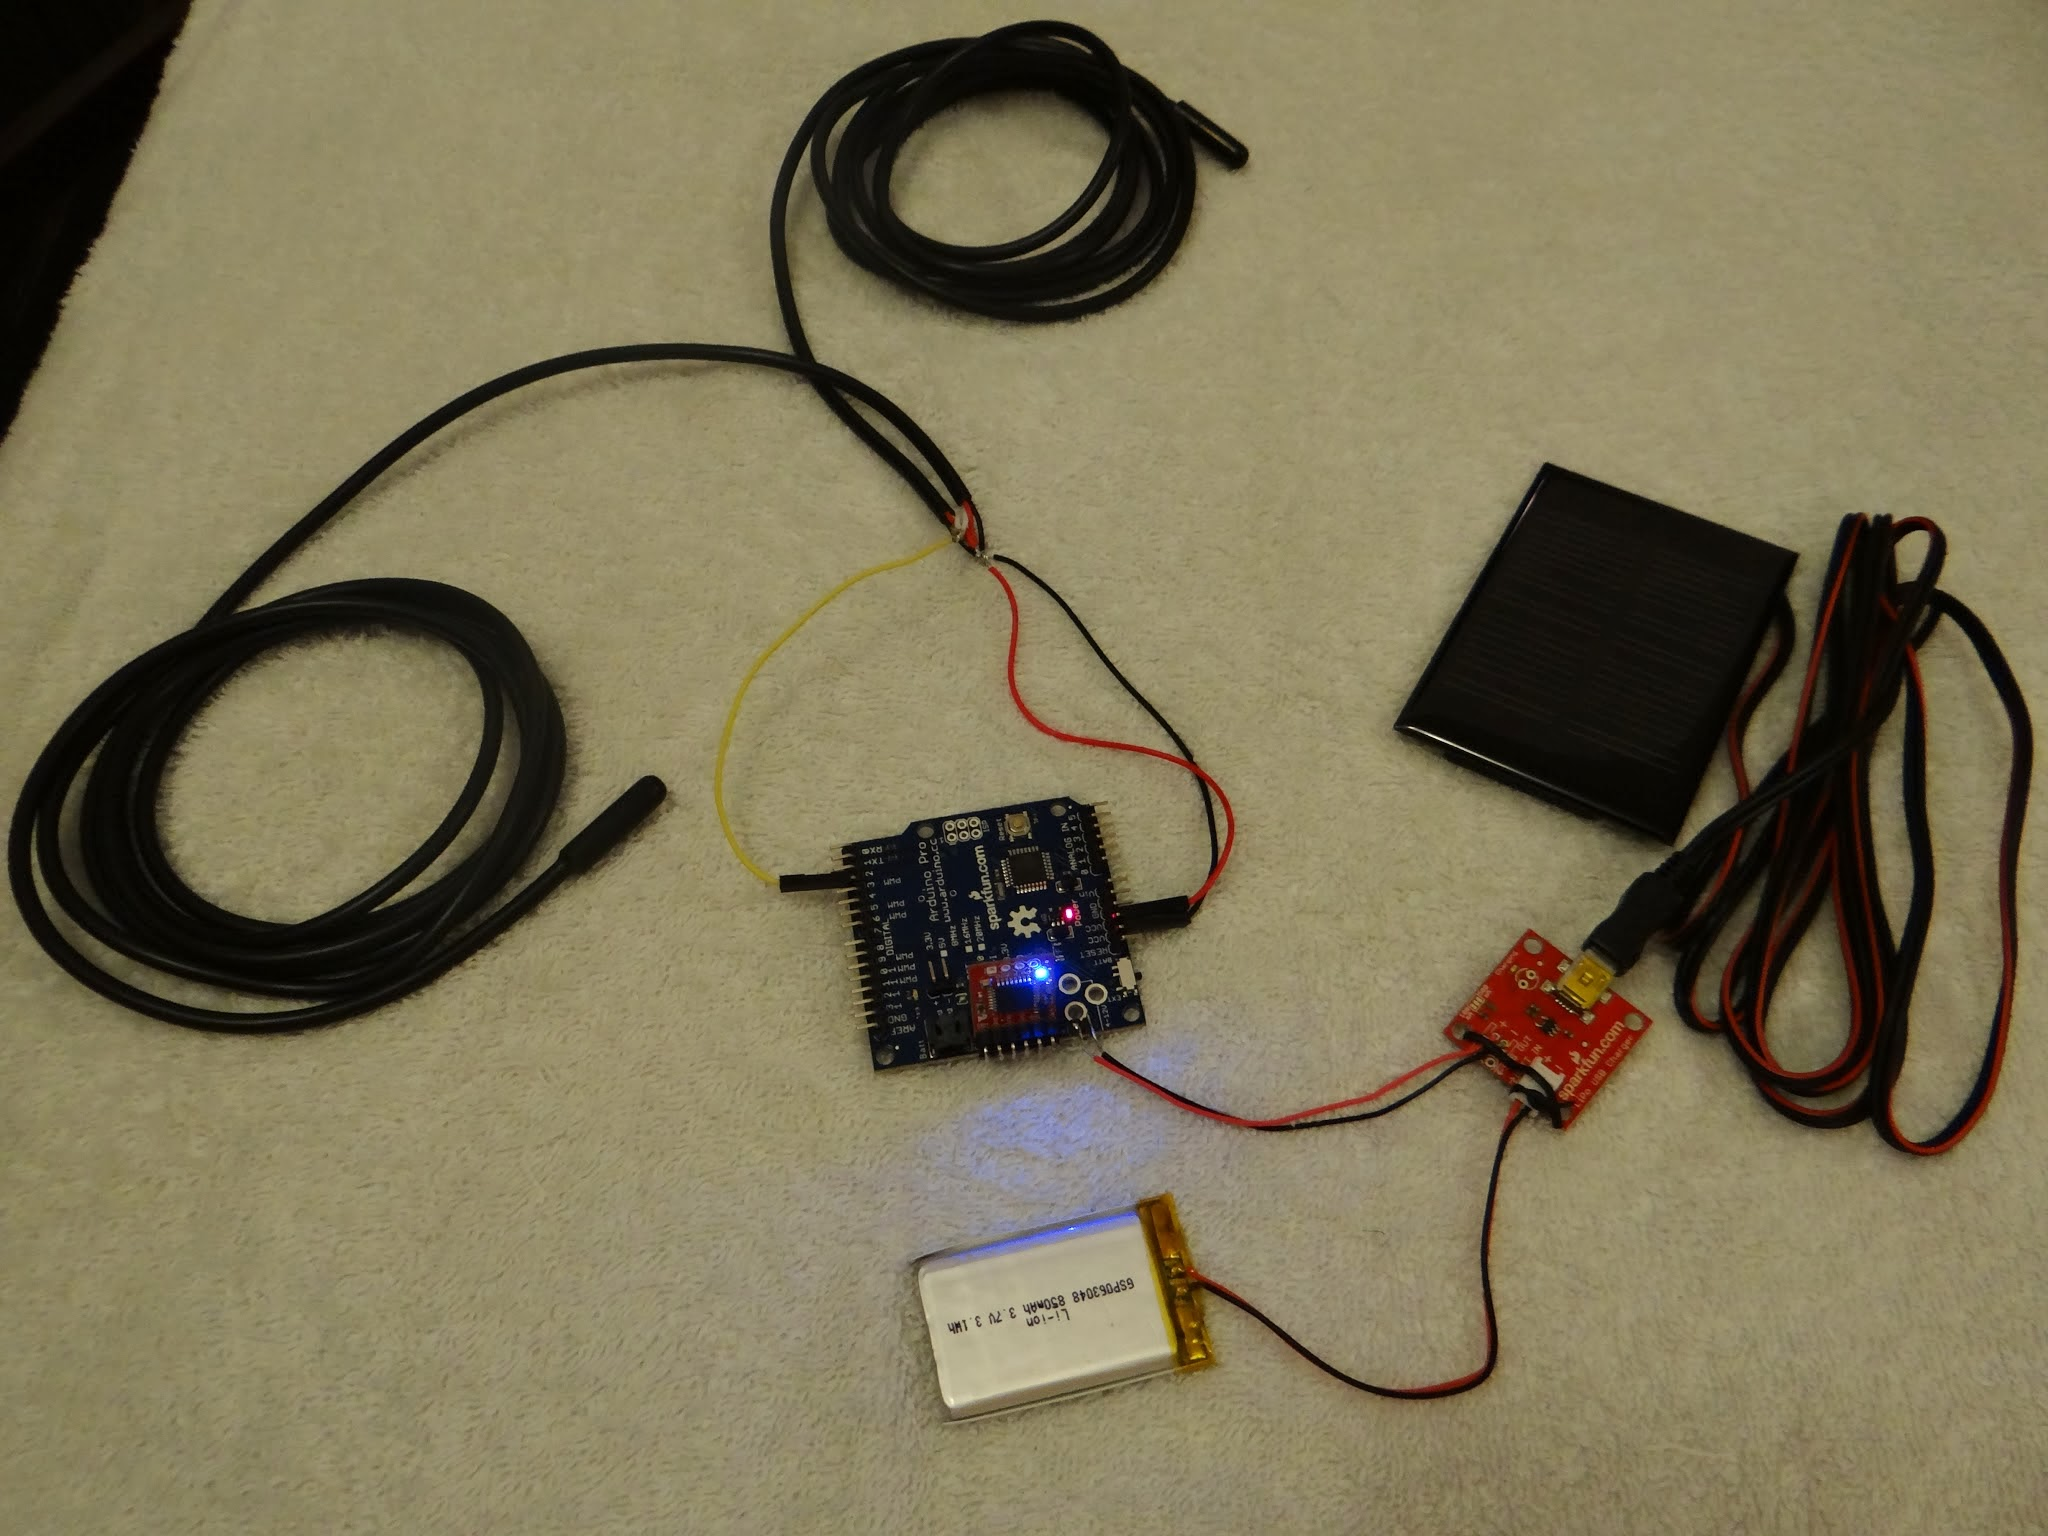
\includegraphics[width=5cm]{MWS}
  \hspace{5mm}
  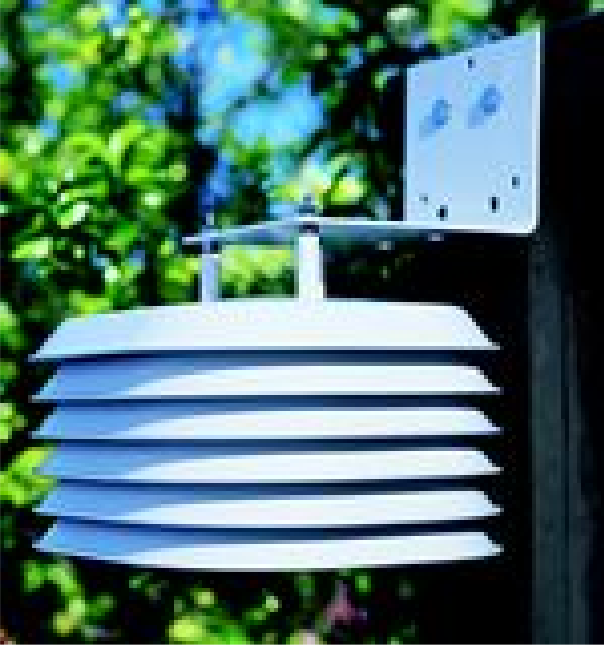
\includegraphics[width=2cm]{MWS_radshield}
\end{flushright}
\end{frame}

\subsection{MWS parts}
%%%%%%%%%%%%%%%%%%%%%%%%%%%%%%%%%%%%%%%%%%%%%%%%%%%%%%%%%%%%%%%%%%%%
{\usebackgroundtemplate{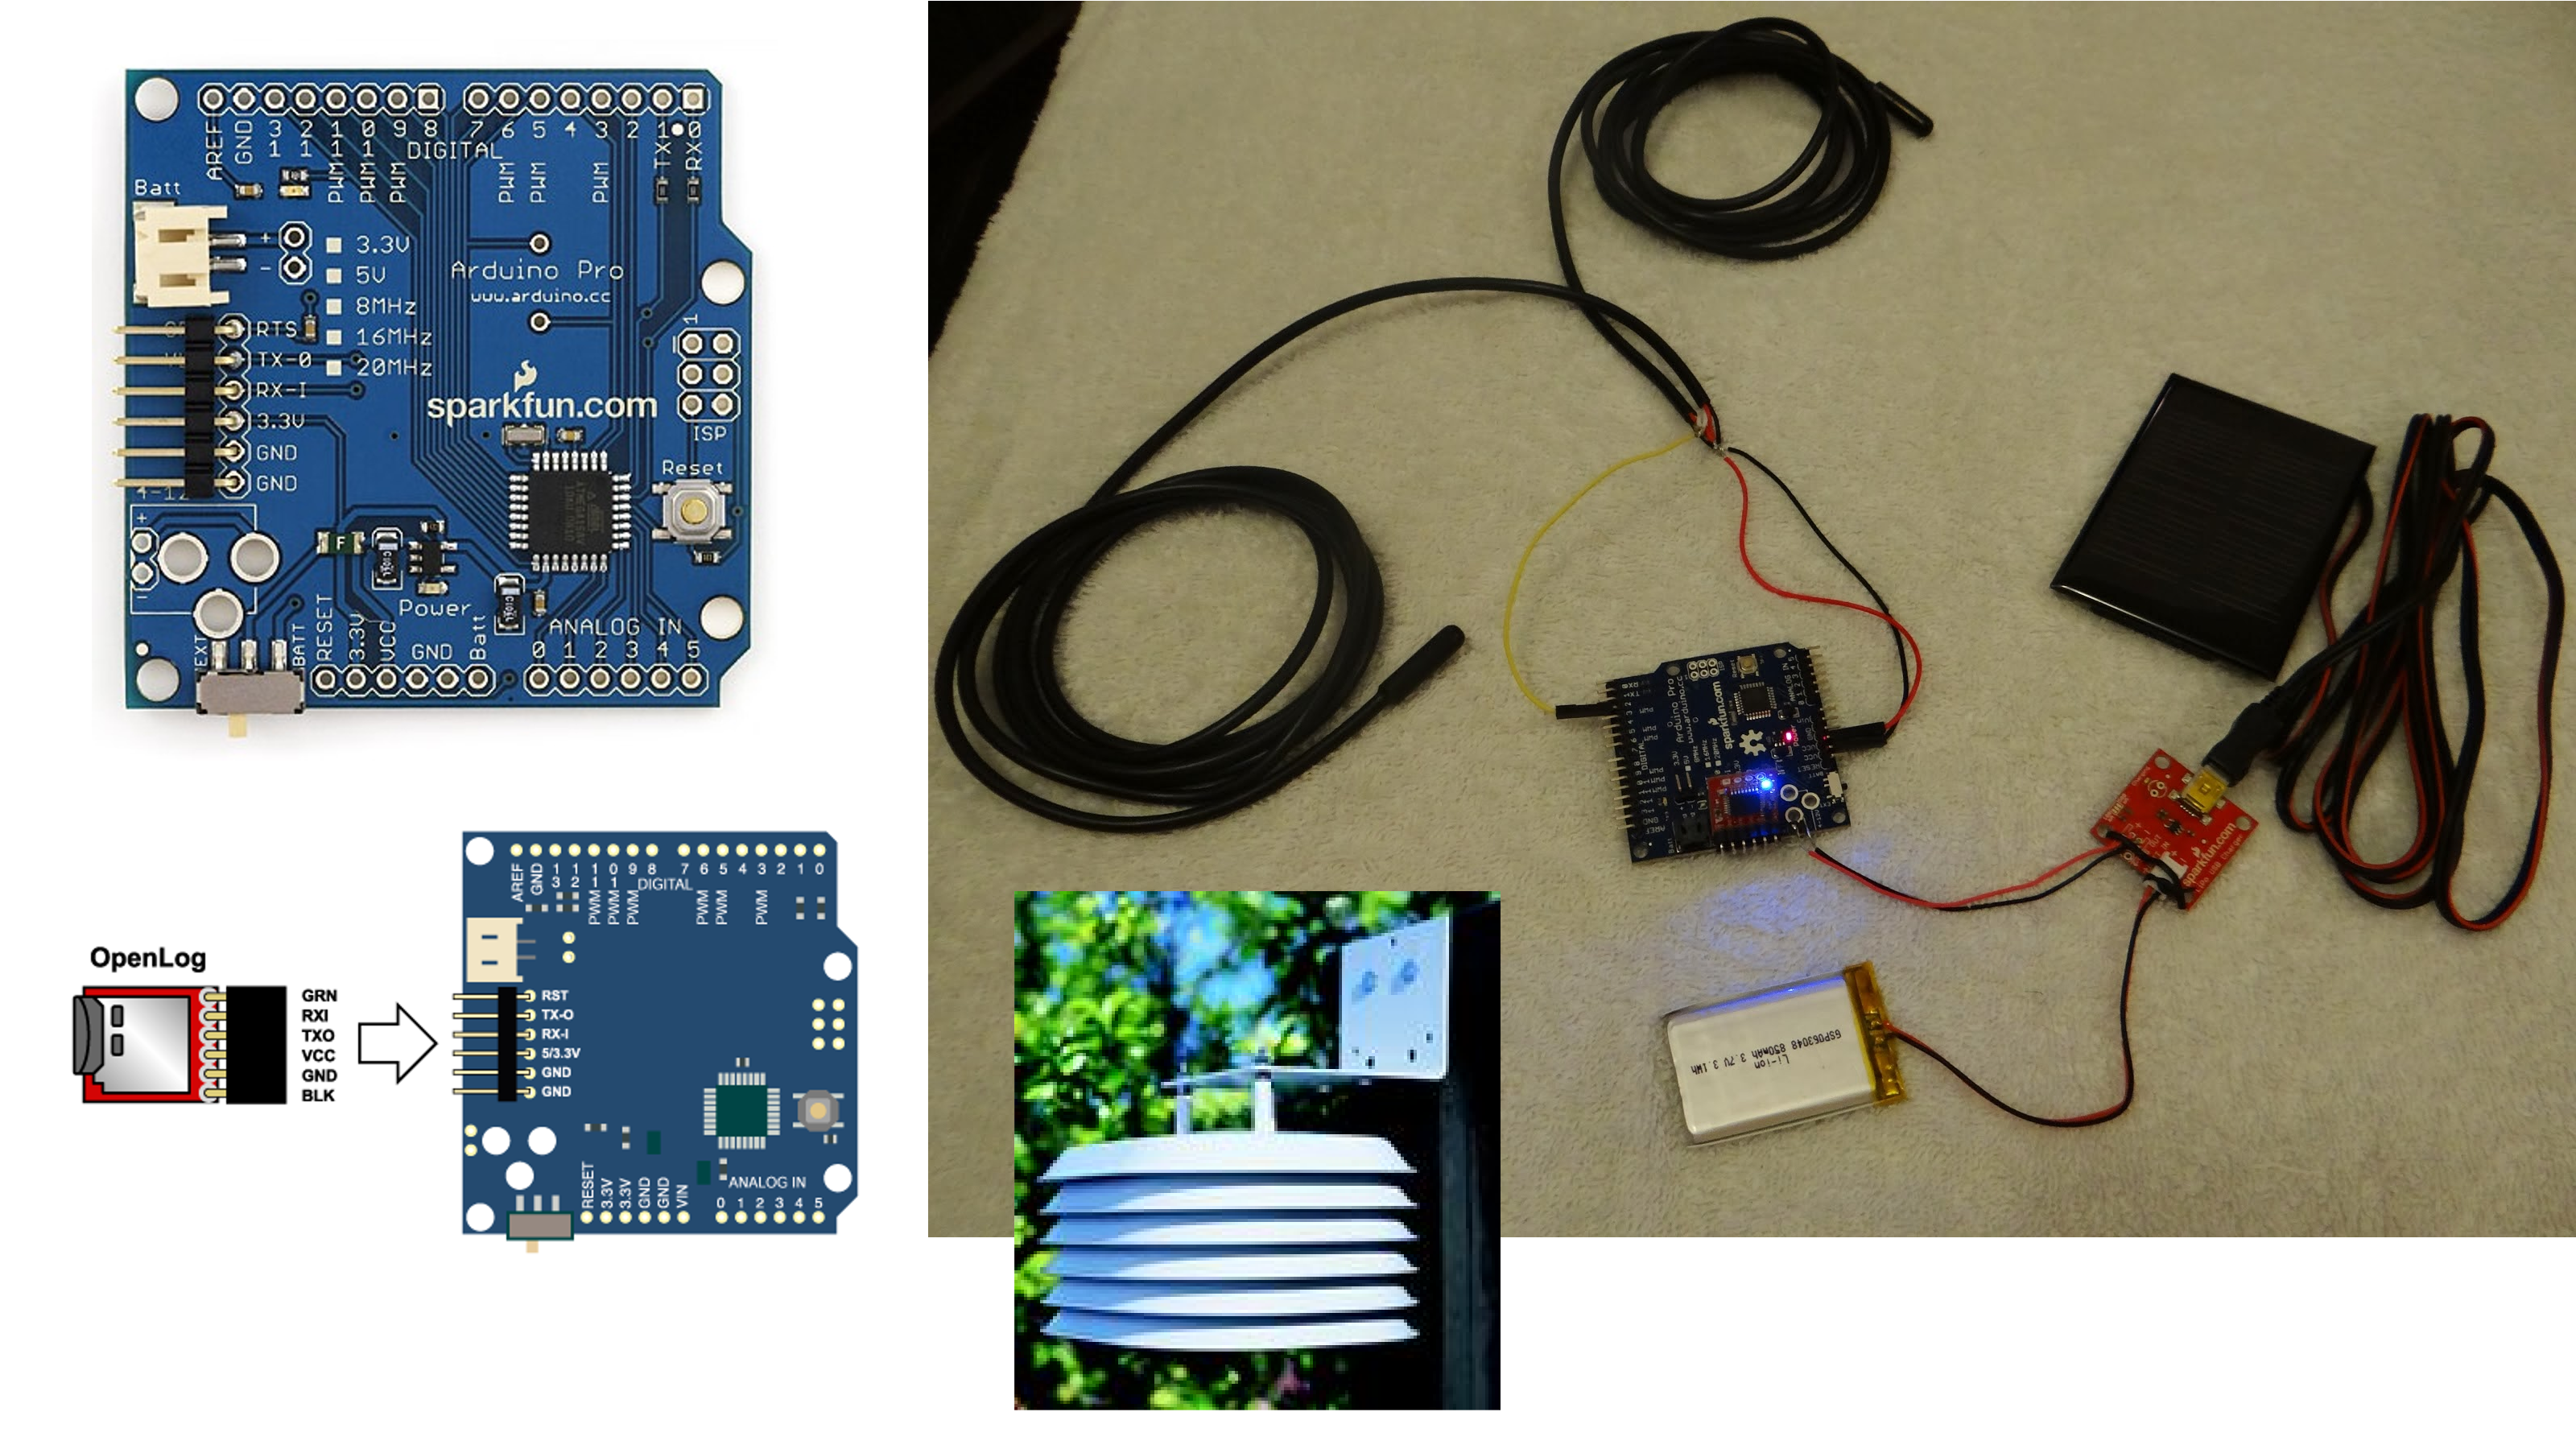
\includegraphics[height=\paperheight,width=\paperwidth]{mwsv1}}
\begin{frame}[plain]
\end{frame}}

\subsection{MWS Setup}
%%%%%%%%%%%%%%%%%%%%%%%%%%%%%%%%%%%%%%%%%%%%%%%%%%%%%%%%%%%%%%%%%%%%
\begin{frame}[fragile]{MWS Setup}

\begin{center}
 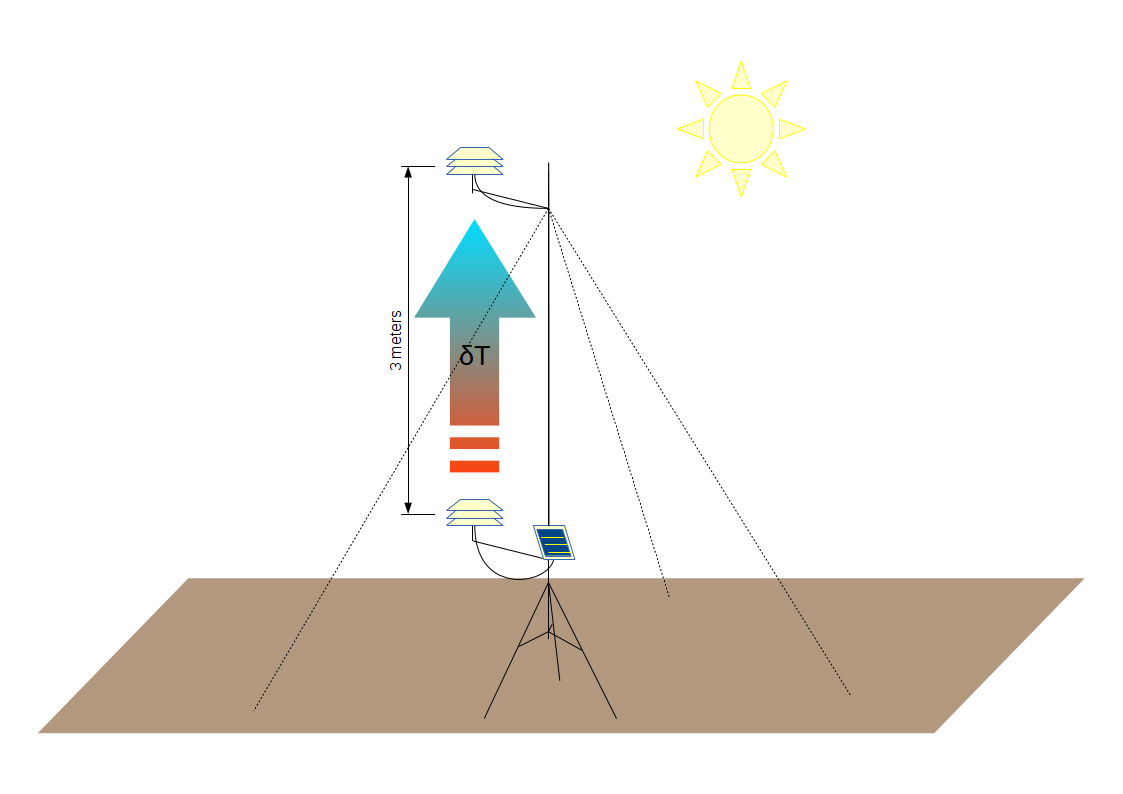
\includegraphics[width=10cm]{MWS_v1_deltaT_sketch_hot}
\end{center}

\end{frame}

%%%%%%%%%%%%%%%%%%%%%%%%%%%%%%%%%%%%%%%%%%%%%%%%%%%%%%%%%%%%%%%%%%%%
\begin{frame}[fragile]{MWS Setup}

\begin{center}
 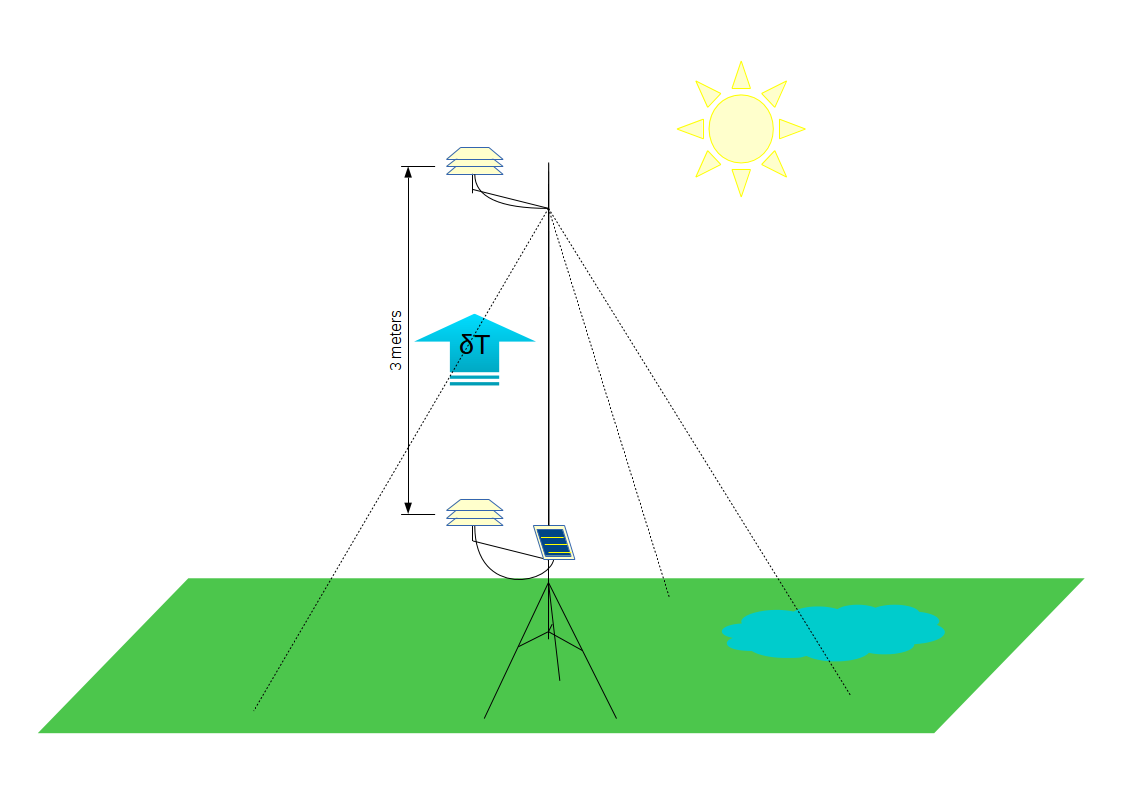
\includegraphics[width=10cm]{MWS_v1_deltaT_sketch_cold}
\end{center}

\end{frame}

%%%%%%%%%%%%%%%%%%%%%%%%%%%%%%%%%%%%%%%%%%%%%%%%%%%%%%%%%%%%%%%%%%%%
{\usebackgroundtemplate{\includegraphics[height=\paperheight,width=\paperwidth]{mwsfieldinstall}}
\begin{frame}[plain]
\end{frame}}


%%%%%%%%%%%%%%%%%%%%%%%%%%%%%%%%%%%%%%%%%%%%%%%%%%%%%%%%%%%%%%%%%%%%
\begin{frame}[plain]
This is nice but what about the lakes, reservoirs, rural tanks?\\
How to calibrate them?
\end{frame}

%%%%%%%%%%%%%%%%%%%%%%%%%%%%%%%%%%%%%%%%%%%%%%%%%%%%%%%%%%%%%%%%%%%%
{\usebackgroundtemplate{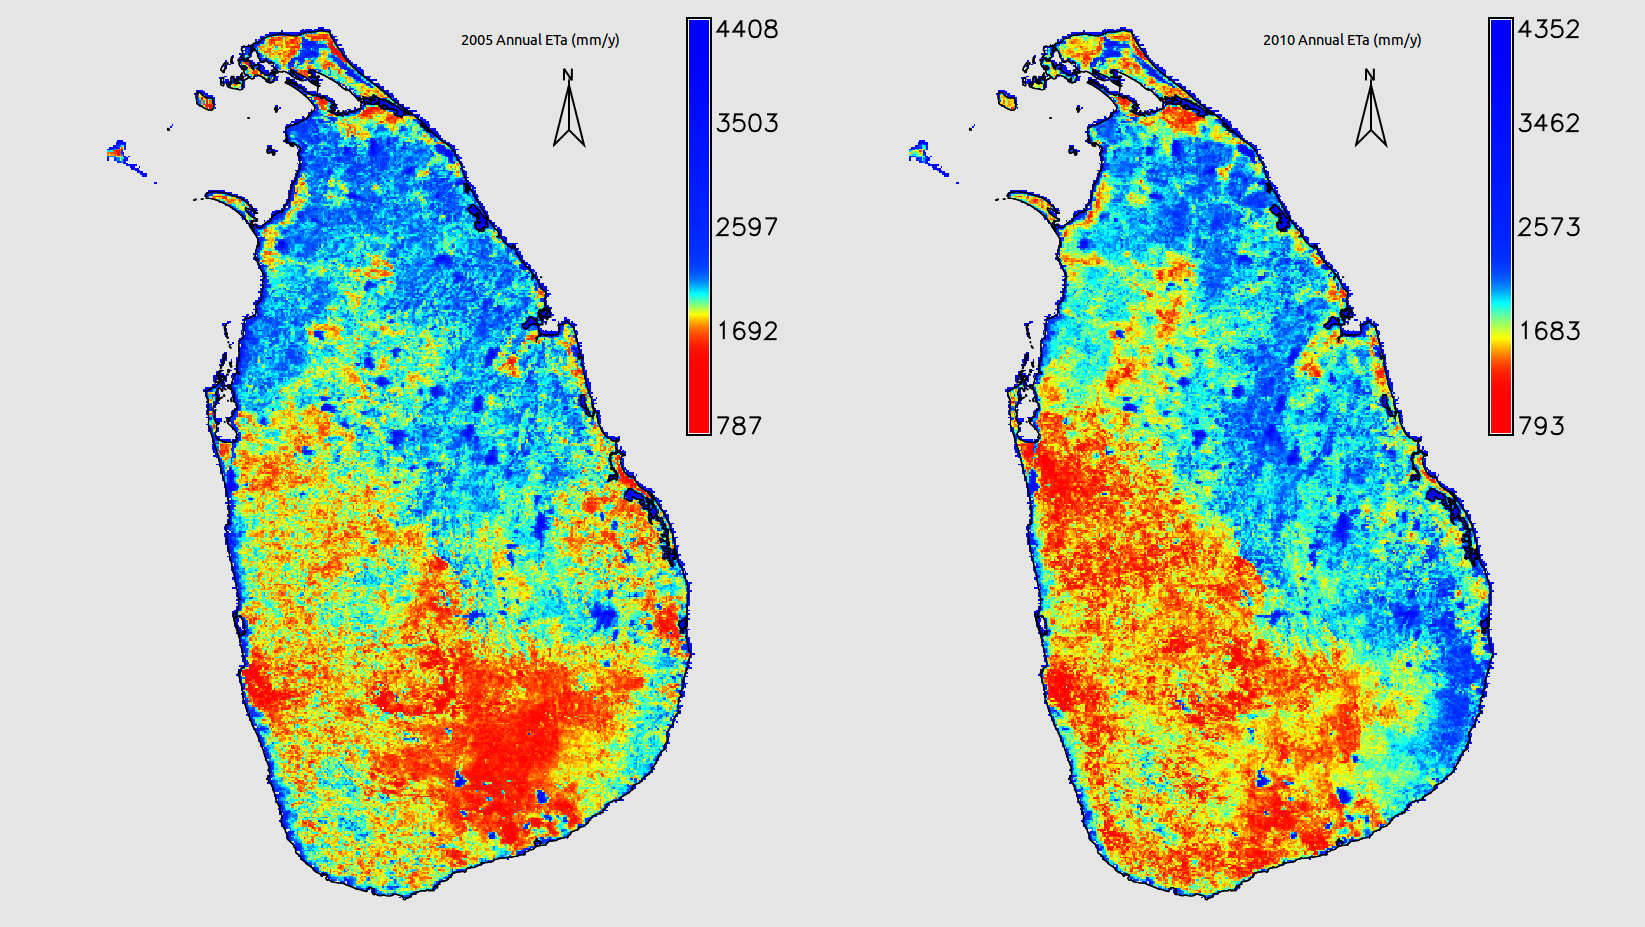
\includegraphics[height=\paperheight,width=\paperwidth]{slet2005_2010}}
\begin{frame}[plain]
\end{frame}}

%%%%%%%%%%%%%%%%%%%%%%%%%%%%%%%%%%%%%%%%%%%%%%%%%%%%%%%%%%%%%%%%%%%%
\begin{frame}[plain]
We need a floating weather station, for few days a year to collect data.
\end{frame}

\section{Amitomi}

\subsection{Autoboat}
%%%%%%%%%%%%%%%%%%%%%%%%%%%%%%%%%%%%%%%%%%%%%%%%%%%%%%%%%%%%%%%%%%%%
\begin{frame}[fragile]{Autonomous Survey Boat}
\textbf{Amitomi} is a 1m-class autonomous sailing boat\\
Designed to survey small tanks temperature gradient for calibrating Evaporation models\\
\vspace{5mm}
{\it \href{https://sites.google.com/site/amitomiautoboat}
{https://sites.google.com/site/amitomiautoboat}}
\begin{columns}
\column[t]{0.5\textwidth}
\begin{center}
 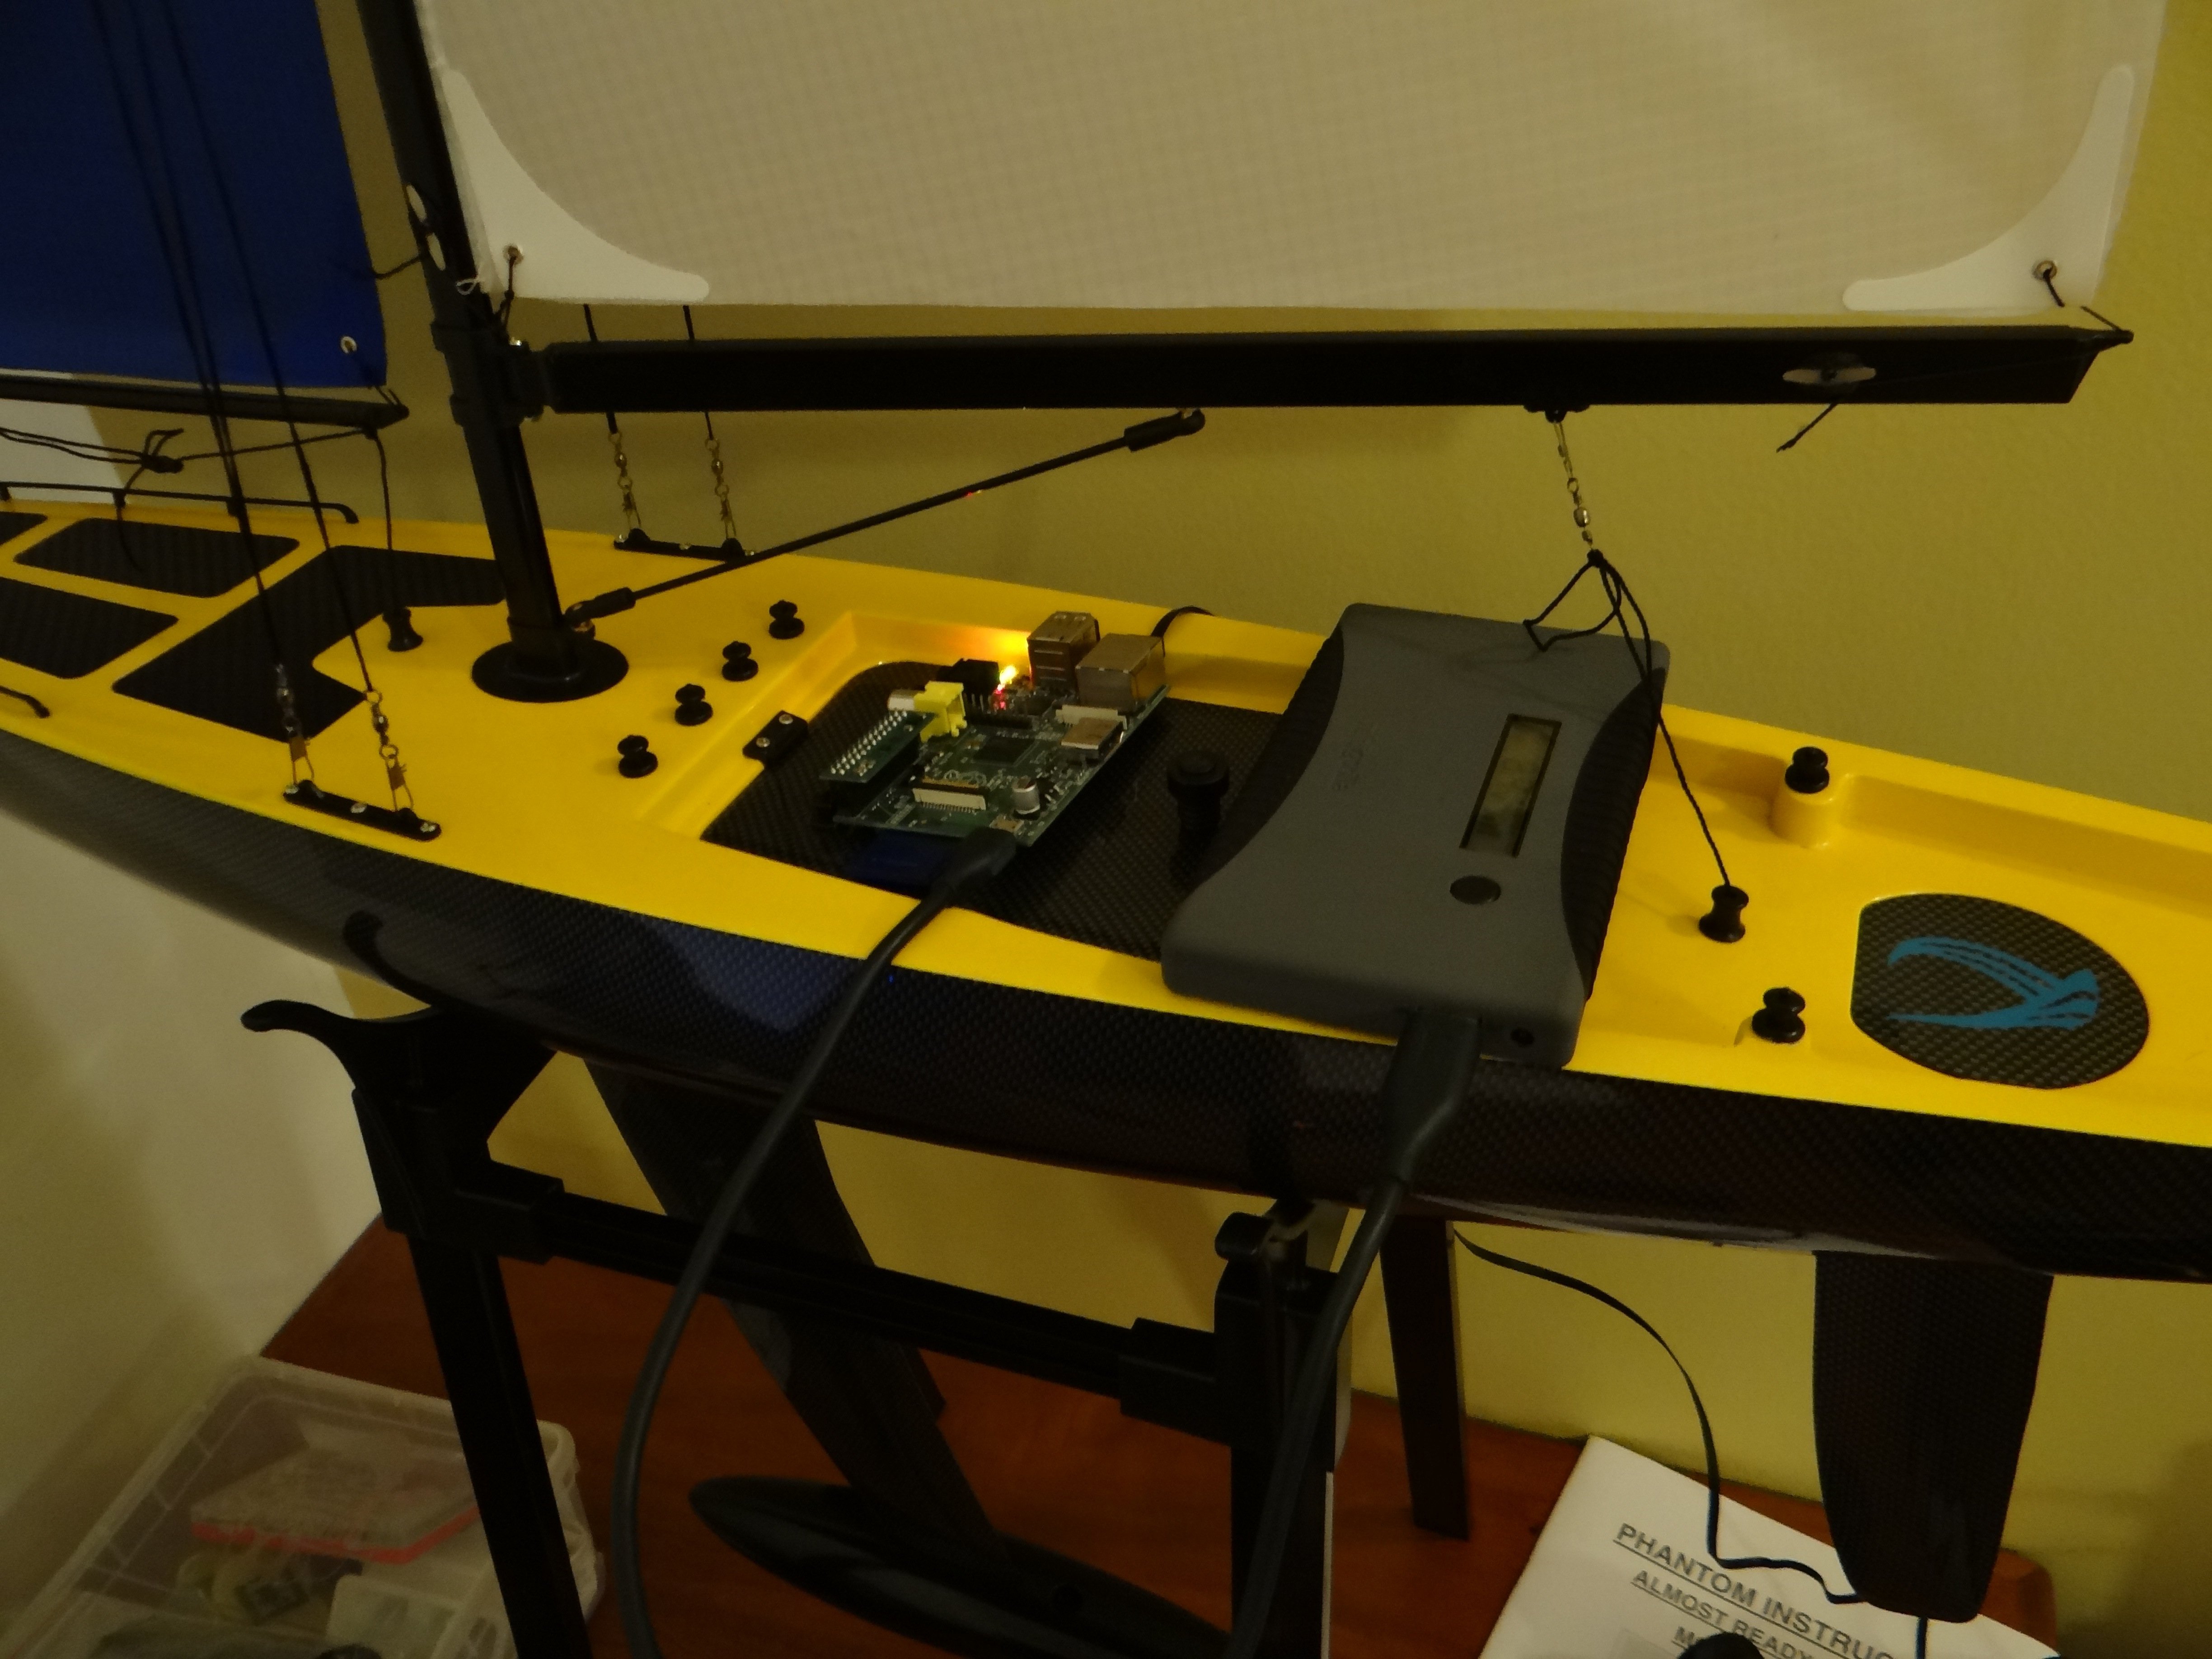
\includegraphics[width=5cm]{sailbot000}
\end{center}
\column[t]{0.5\textwidth}
\begin{center}
 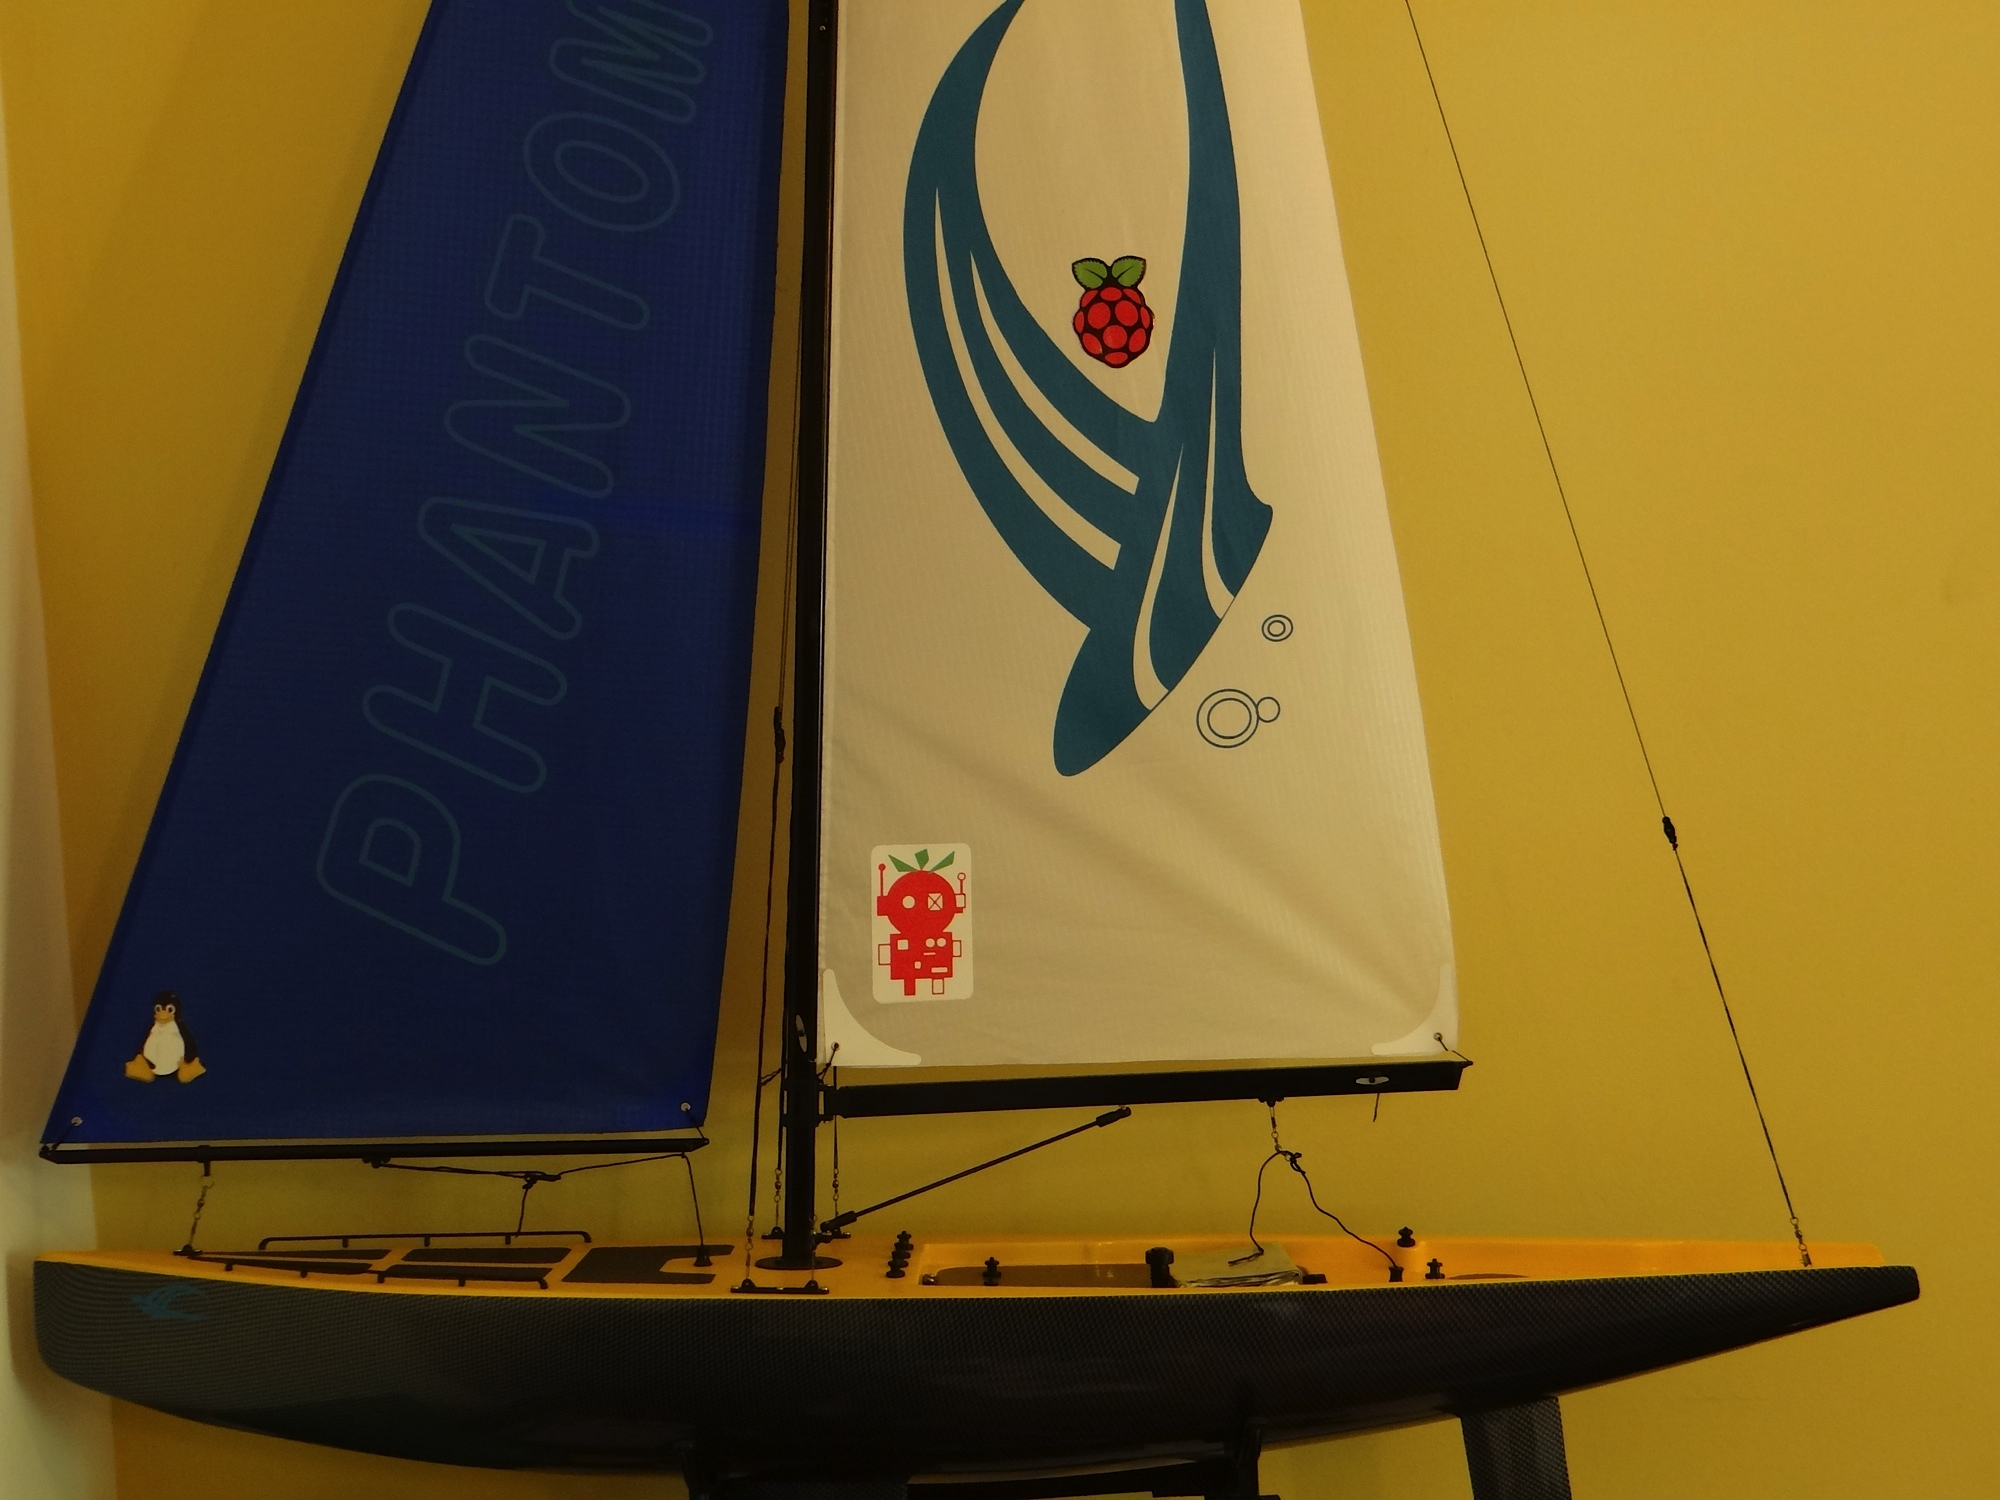
\includegraphics[width=5cm]{sailbot001}
\end{center}
\end{columns}
\end{frame}

%%%%%%%%%%%%%%%%%%%%%%%%%%%%%%%%%%%%%%%%%%%%%%%%%%%%%%%%%%%%%%%%%%%%
{\usebackgroundtemplate{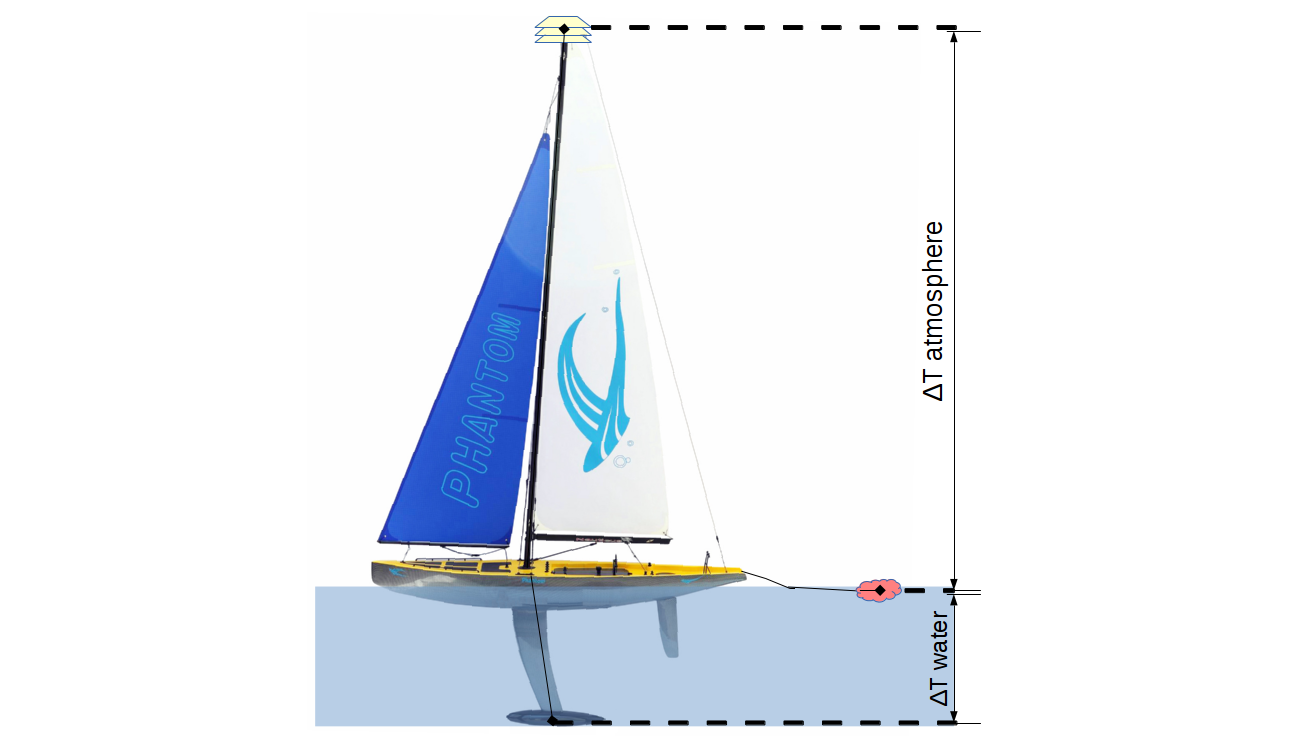
\includegraphics[height=\paperheight,width=\paperwidth]{amitomiv1}}
\begin{frame}[plain]
\end{frame}}

\subsection{Components}
%%%%%%%%%%%%%%%%%%%%%%%%%%%%%%%%%%%%%%%%%%%%%%%%%%%%%%%%%%%%%%%%%%%%
\begin{frame}[fragile]{Details}
\begin{columns}
\column[t]{0.4\textwidth}
\textbf{Components}
\vspace{5mm}
\begin{itemize}
 \item RaspberryPI v2
 \item + XloBorg Accelerometer
 \item + GPS shield
 \item + motor shield
 \item + Python code
\end{itemize}
\column[t]{0.6\textwidth}
\begin{center}
 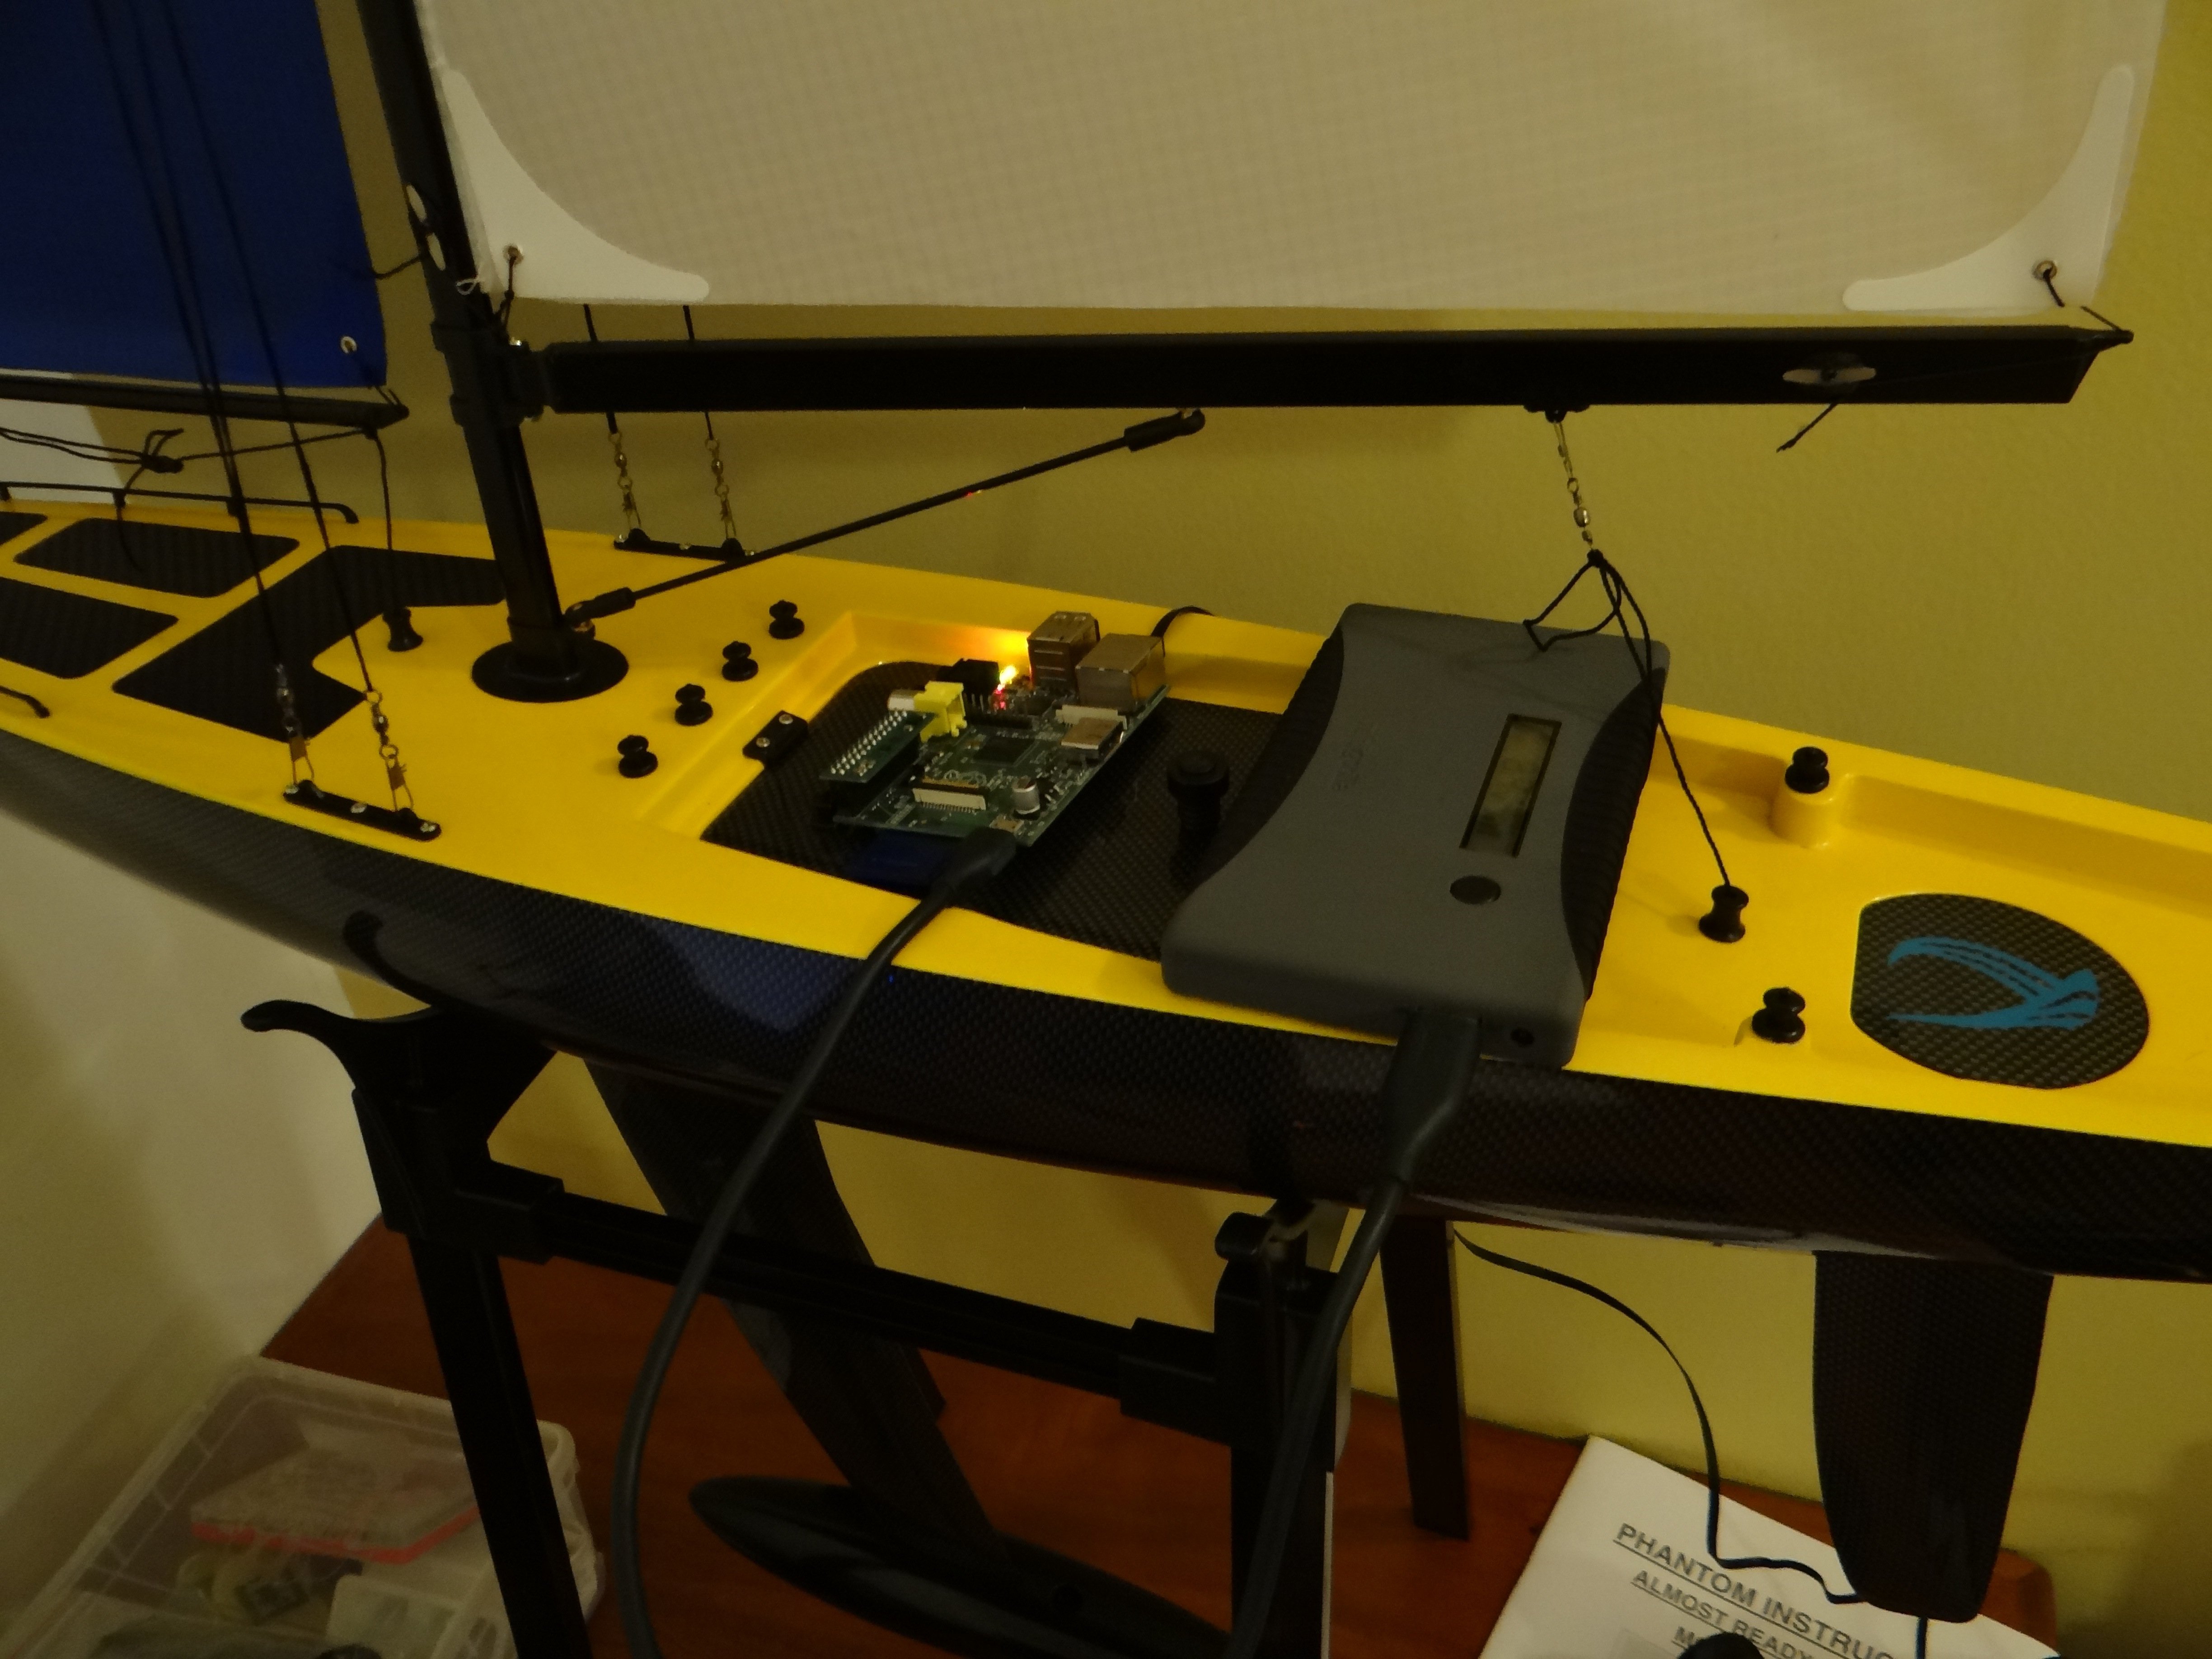
\includegraphics[width=8cm]{sailbot000}
\end{center}
\end{columns}
\end{frame}

%%%%%%%%%%%%%%%%%%%%%%%%%%%%%%%%%%%%%%%%%%%%%%%%%%%%%%%%%%%%%%%%%%%%
{\usebackgroundtemplate{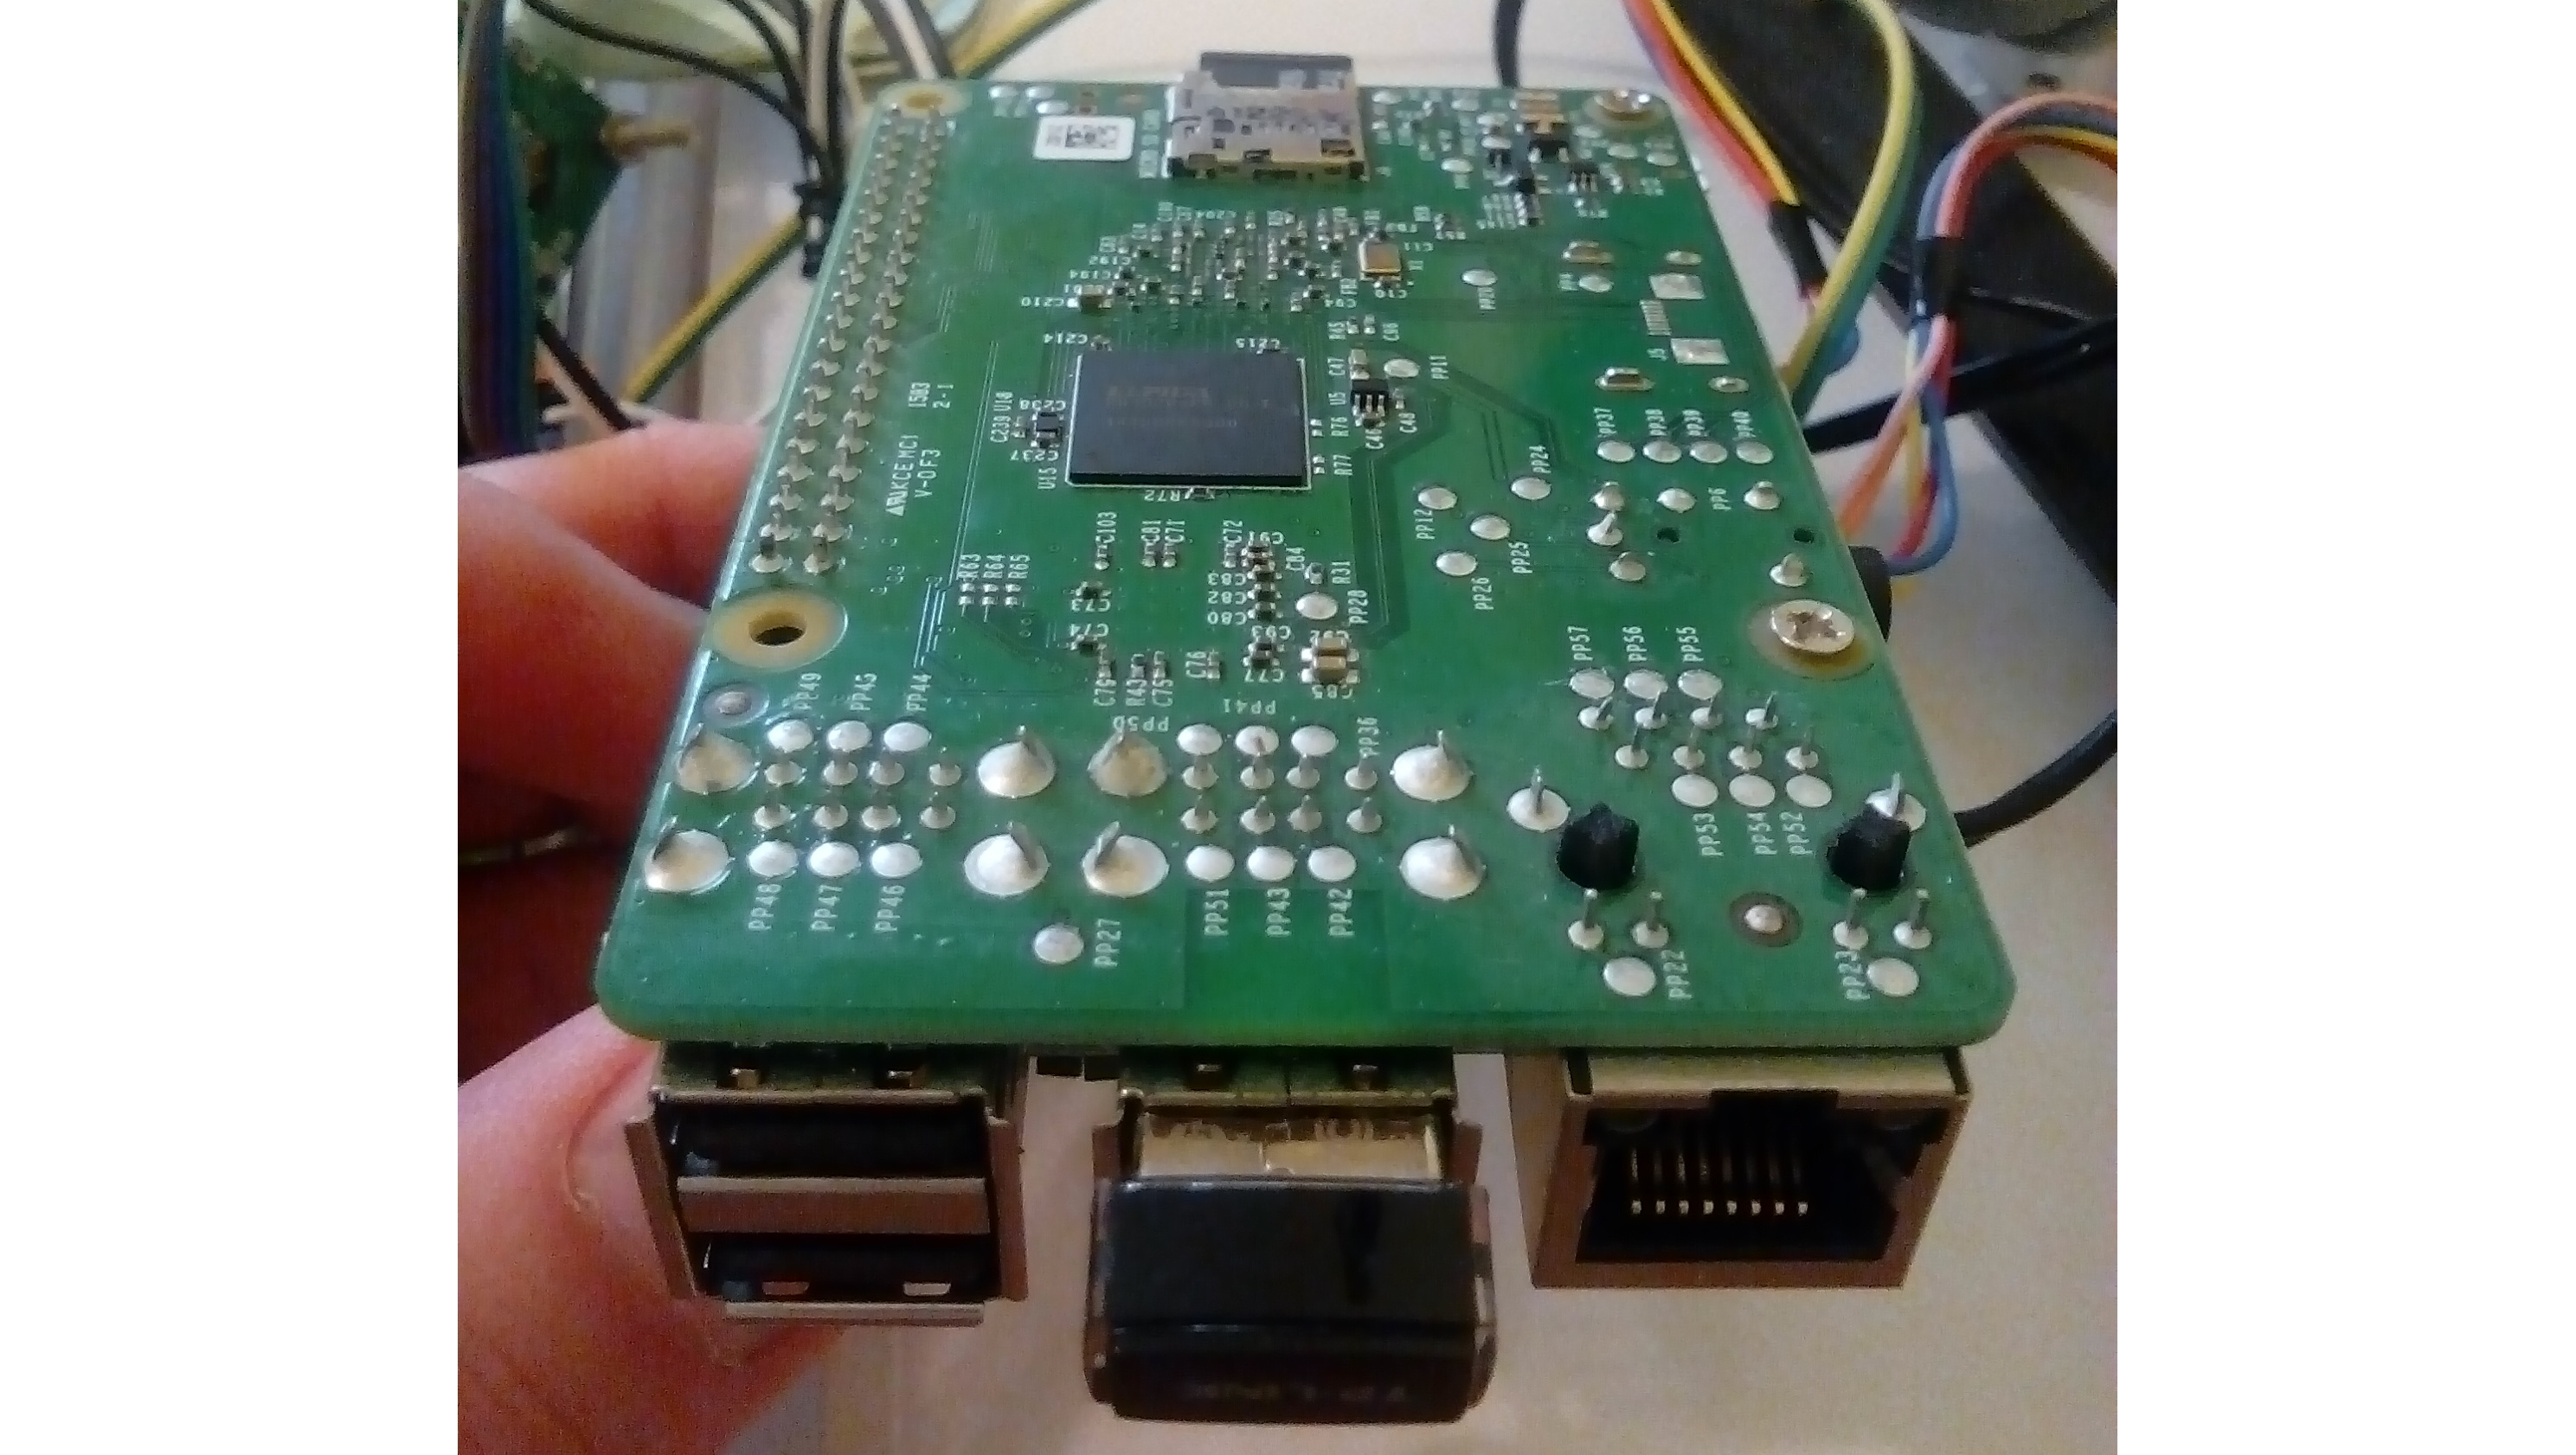
\includegraphics[height=\paperheight,width=\paperwidth]{rpiv2}}
\begin{frame}[plain]
\end{frame}}

%%%%%%%%%%%%%%%%%%%%%%%%%%%%%%%%%%%%%%%%%%%%%%%%%%%%%%%%%%%%%%%%%%%%
{\usebackgroundtemplate{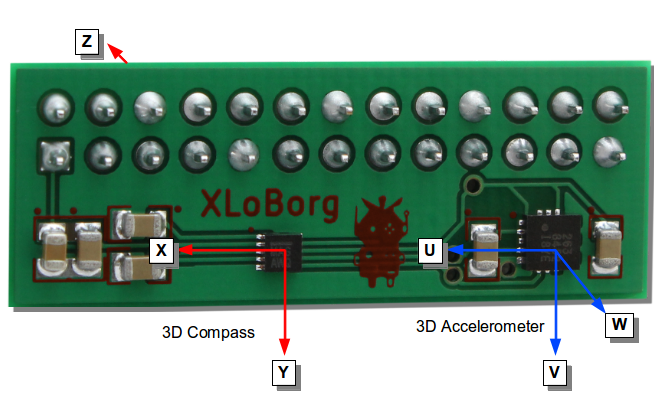
\includegraphics[height=\paperheight,width=\paperwidth]{xloborg_axis_details}}
\begin{frame}[plain]
\end{frame}}

\subsection{Compass/Accelerometer}
%%%%%%%%%%%%%%%%%%%%%%%%%%%%%%%%%%%%%%%%%%%%%%%%%%%%%%%%%%%%%%%%%%%%
\begin{frame}[fragile]{Compass/Accelerometer}
\begin{columns}
\column[t]{0.4\textwidth}
\textbf{Compass/Accelerometer software}
\vspace{5mm}
\begin{itemize}
 \item Python - XloBorg 
 \item 3D Compass
 \item 3D Accelerometer
 \item Pitch/Yaw/Roll
 \item Azimuth (for Bearing)
 \end{itemize}
\column[t]{0.6\textwidth}
\begin{center}
 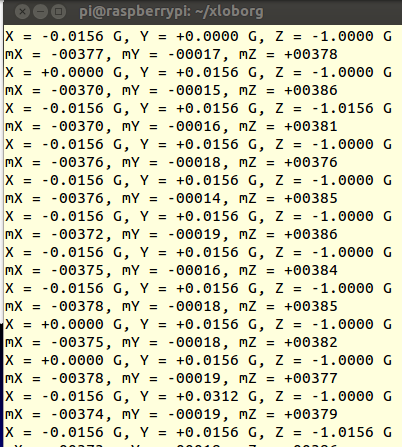
\includegraphics[width=7cm]{accelerometer_data}
\end{center}
\end{columns}
\end{frame}

\subsection{Attitude}
%%%%%%%%%%%%%%%%%%%%%%%%%%%%%%%%%%%%%%%%%%%%%%%%%%%%%%%%%%%%%%%%%%%%
\begin{frame}[fragile]{Attitude}
\begin{columns}
\column[t]{0.3\textwidth}
\textbf{Attitude software}
\vspace{5mm}
\begin{itemize}
 \item Python - XloBorg 
 \item 3D Compass
 \item 3D Accelerometer
 \item Pitch/Yaw/Roll
 \item Attitude of the boat
 \end{itemize}
\column[t]{0.7\textwidth}
\begin{center}
 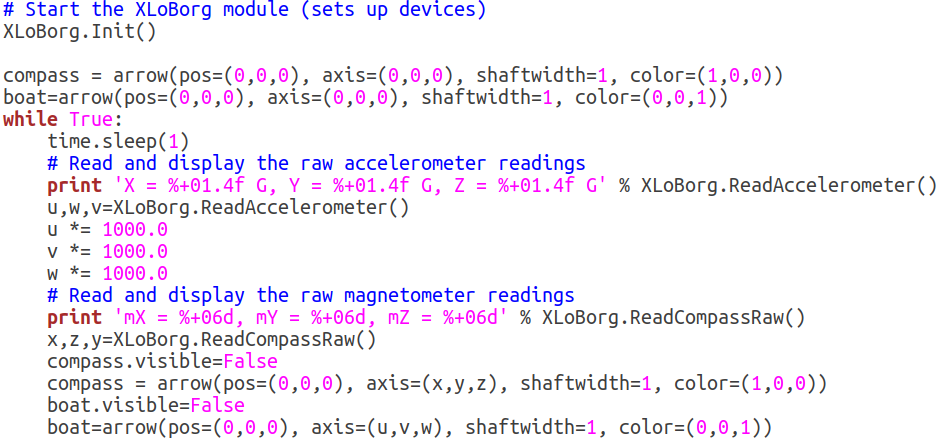
\includegraphics[width=10cm]{attitude_py}
\end{center}
\end{columns}
\end{frame}

%%%%%%%%%%%%%%%%%%%%%%%%%%%%%%%%%%%%%%%%%%%%%%%%%%%%%%%%%%%%%%%%%%%%
{\usebackgroundtemplate{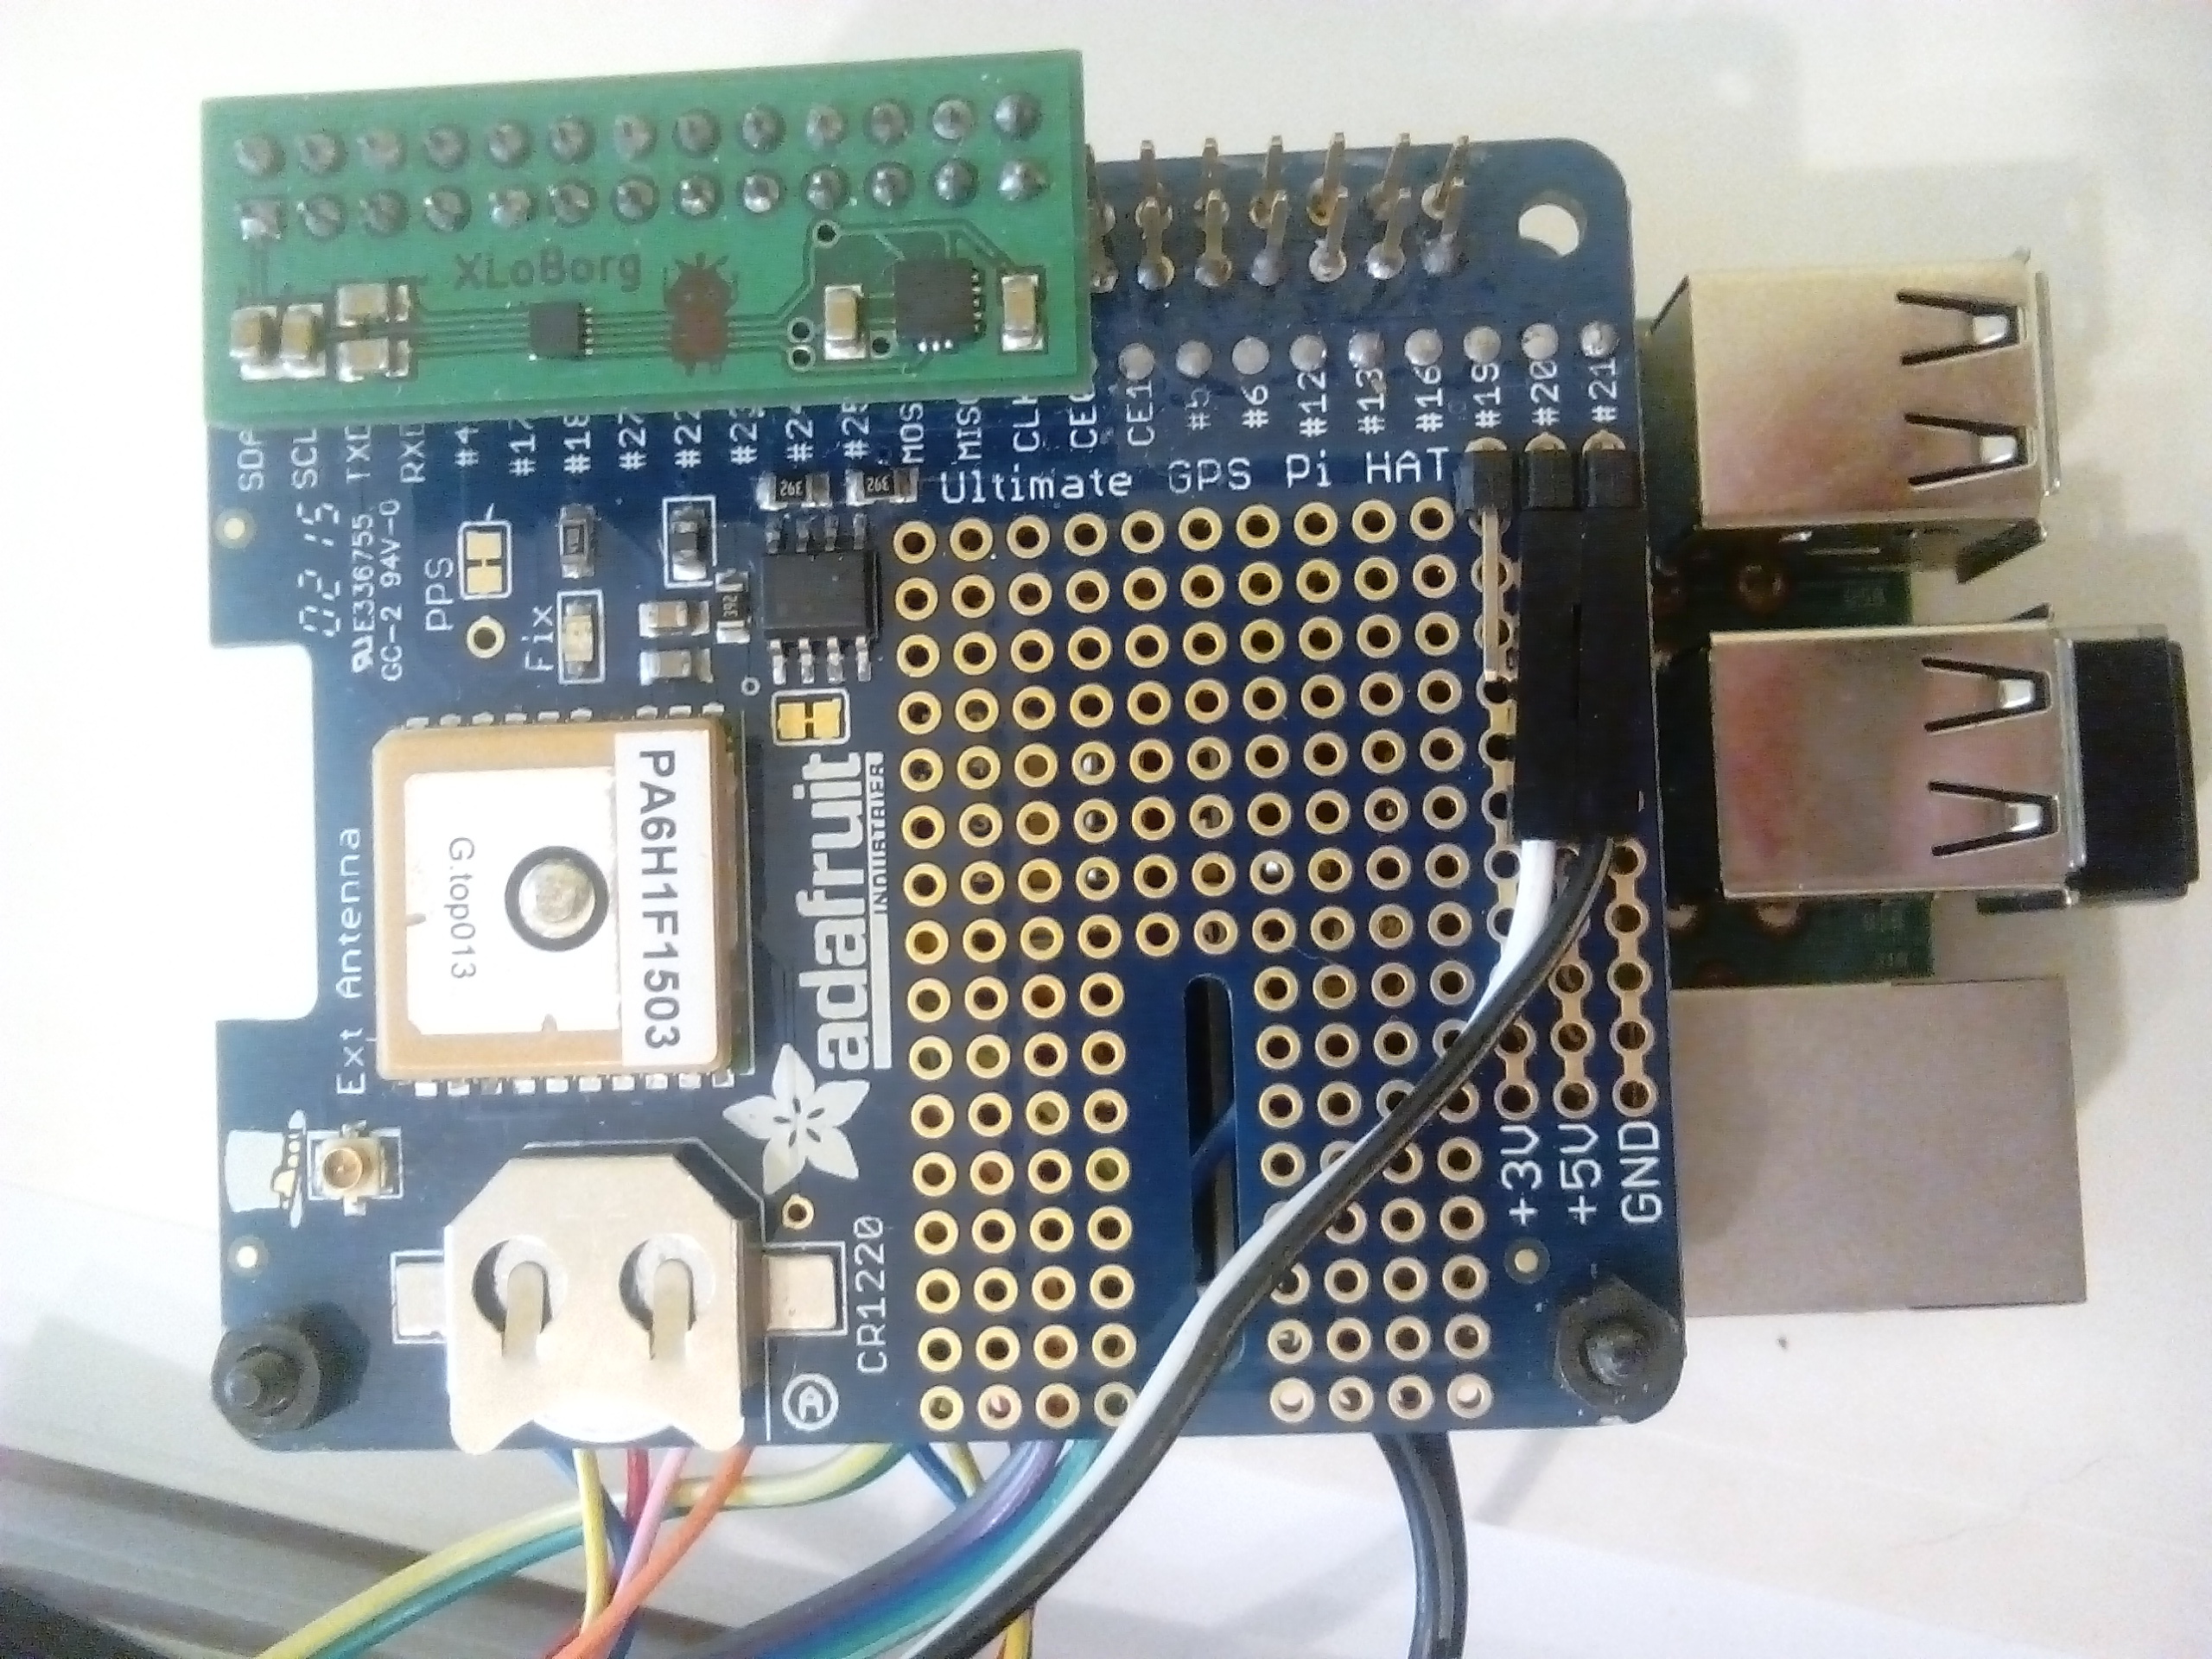
\includegraphics[height=\paperheight,width=\paperwidth]{gpsshield}}
\begin{frame}[plain]
\end{frame}}

\subsection{GPS/Bearing}
%%%%%%%%%%%%%%%%%%%%%%%%%%%%%%%%%%%%%%%%%%%%%%%%%%%%%%%%%%%%%%%%%%%%
\begin{frame}[fragile]{GPS/Bearing}
\begin{columns}
\column[t]{0.3\textwidth}
\textbf{GPS/Bearing software}
\vspace{5mm}
\begin{itemize}
 \item Python - GPS 
 \item GPS RPIv2 Hat
 \item Location
 \item Azimuth (for Bearing)
 \end{itemize}
\column[t]{0.7\textwidth}
\begin{center}
 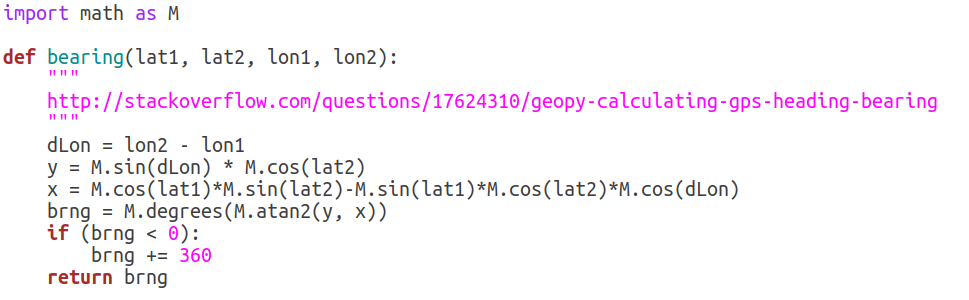
\includegraphics[width=10.5cm]{bearing_py}
\end{center}
\end{columns}
\end{frame}

%%%%%%%%%%%%%%%%%%%%%%%%%%%%%%%%%%%%%%%%%%%%%%%%%%%%%%%%%%%%%%%%%%%%
{\usebackgroundtemplate{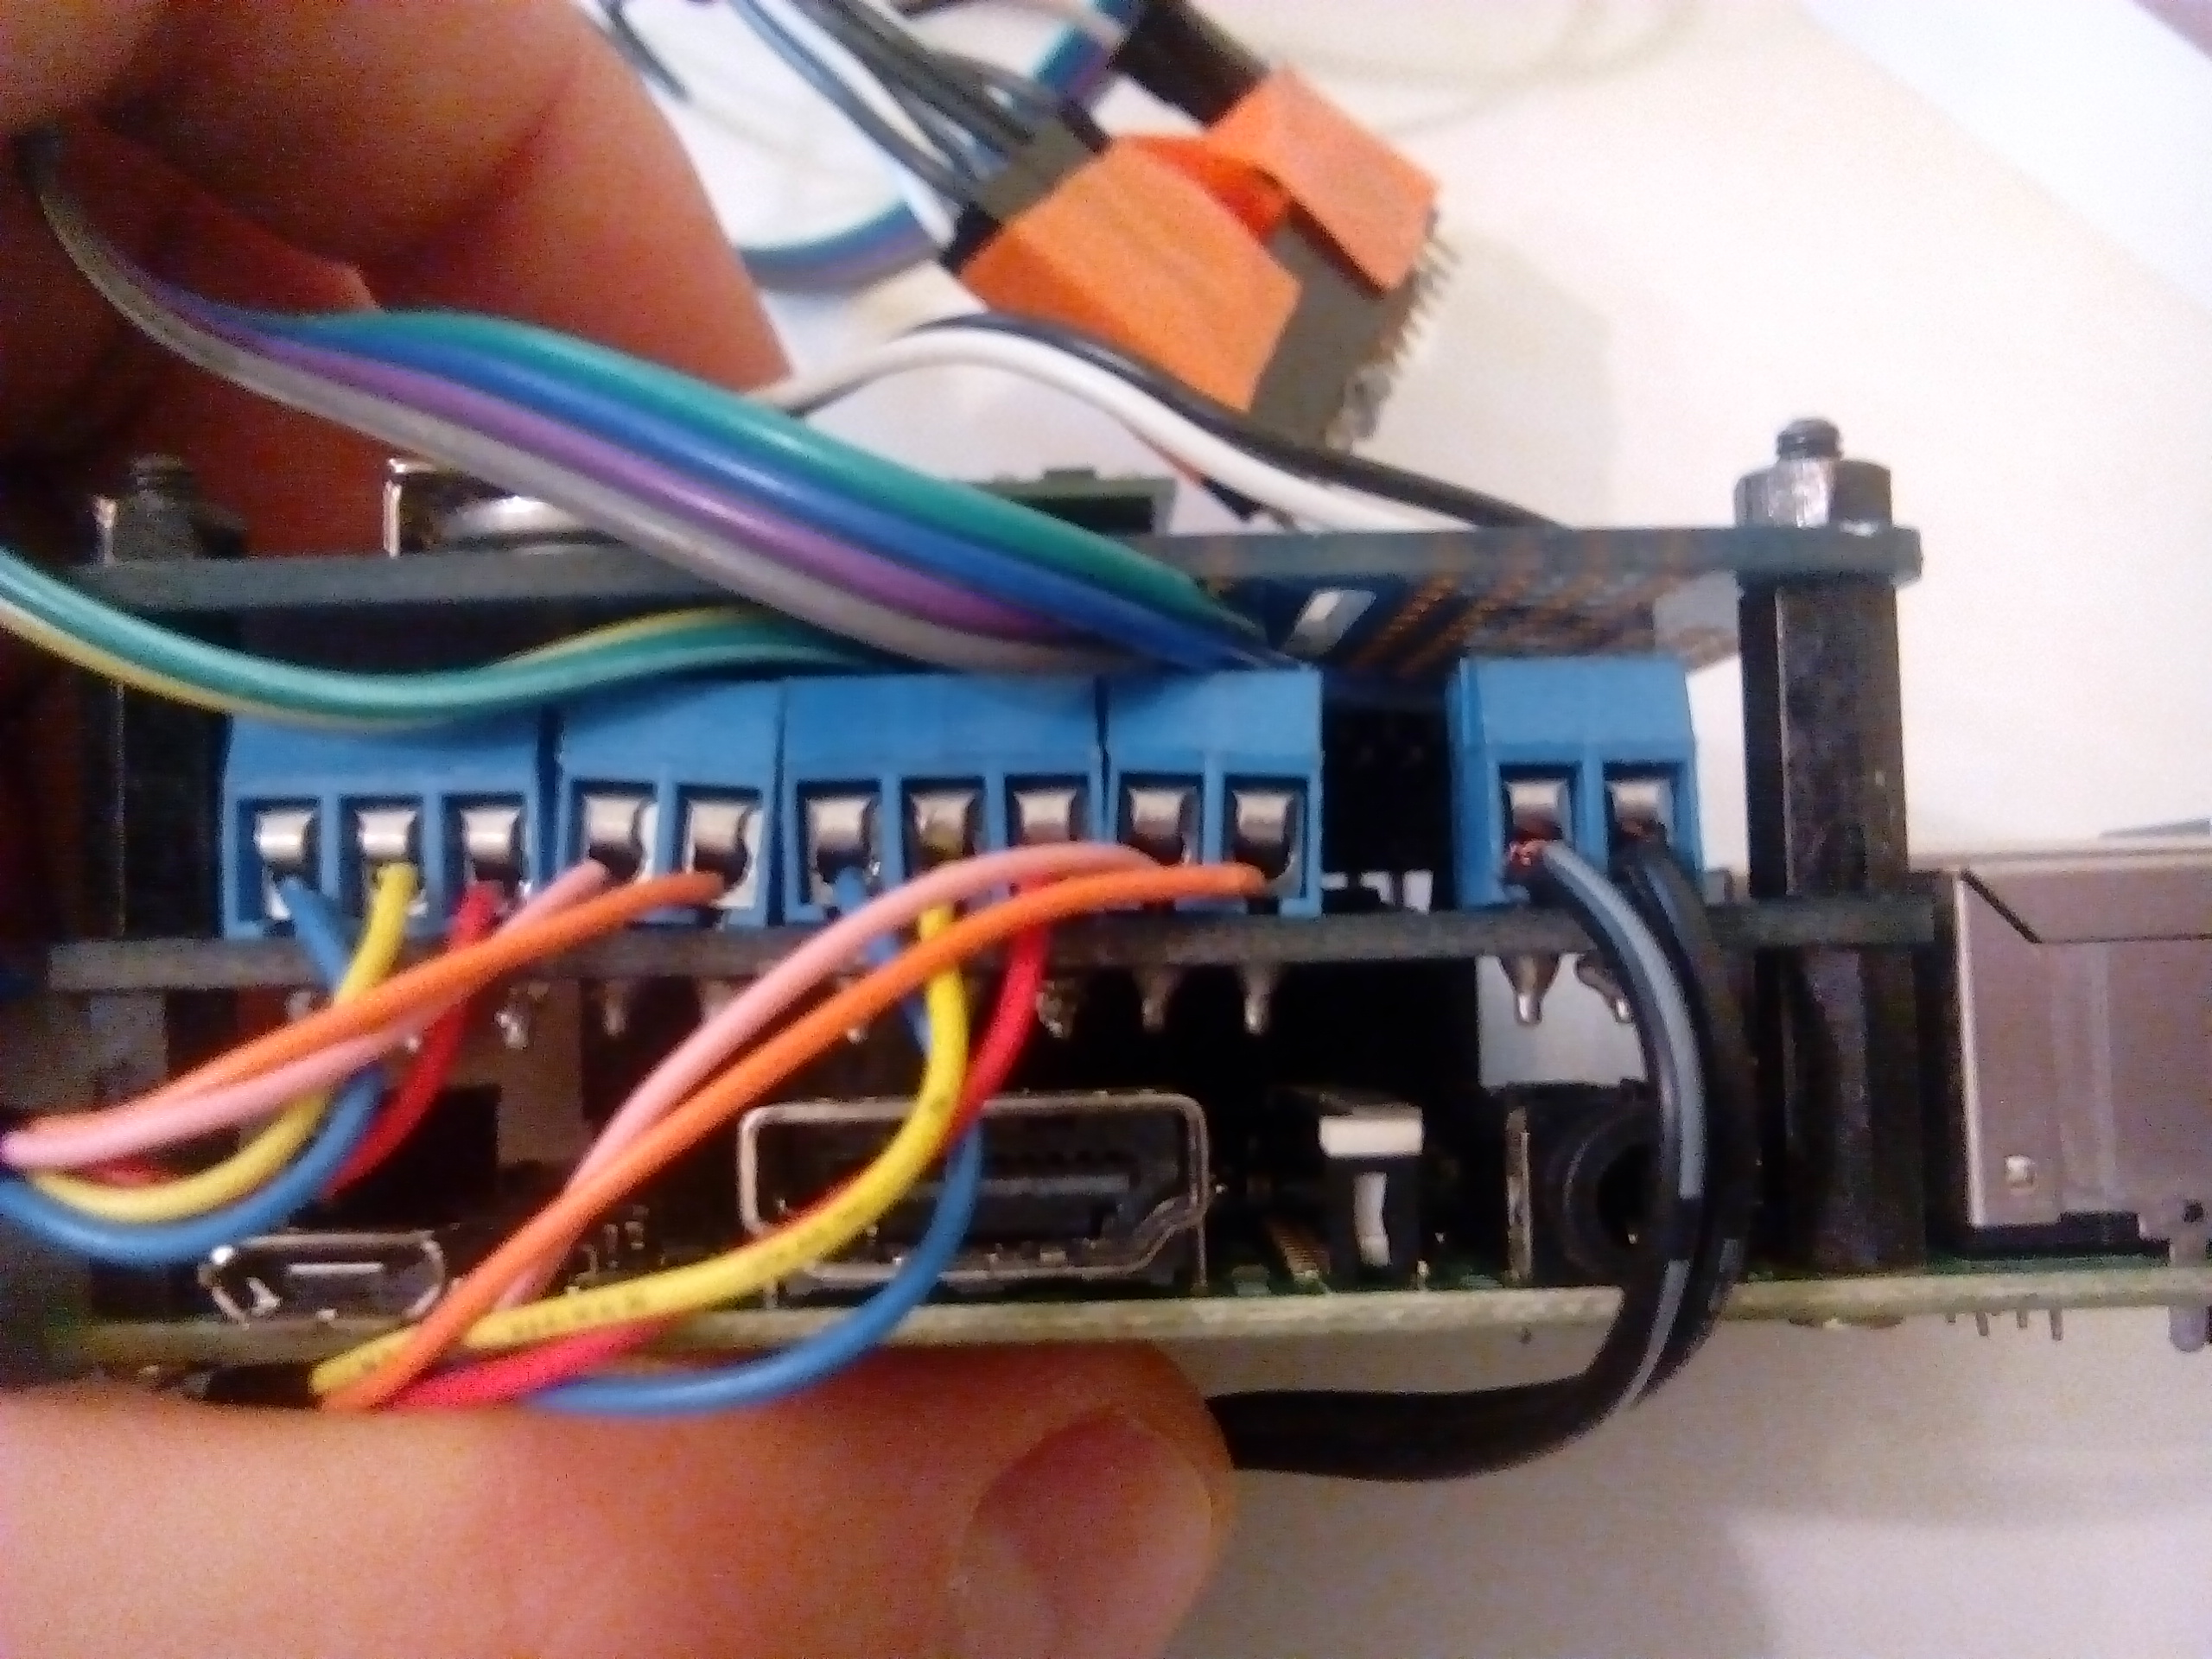
\includegraphics[height=\paperheight,width=\paperwidth]{motorshield}}
\begin{frame}[plain]
\end{frame}}

%%%%%%%%%%%%%%%%%%%%%%%%%%%%%%%%%%%%%%%%%%%%%%%%%%%%%%%%%%%%%%%%%%%%
{\usebackgroundtemplate{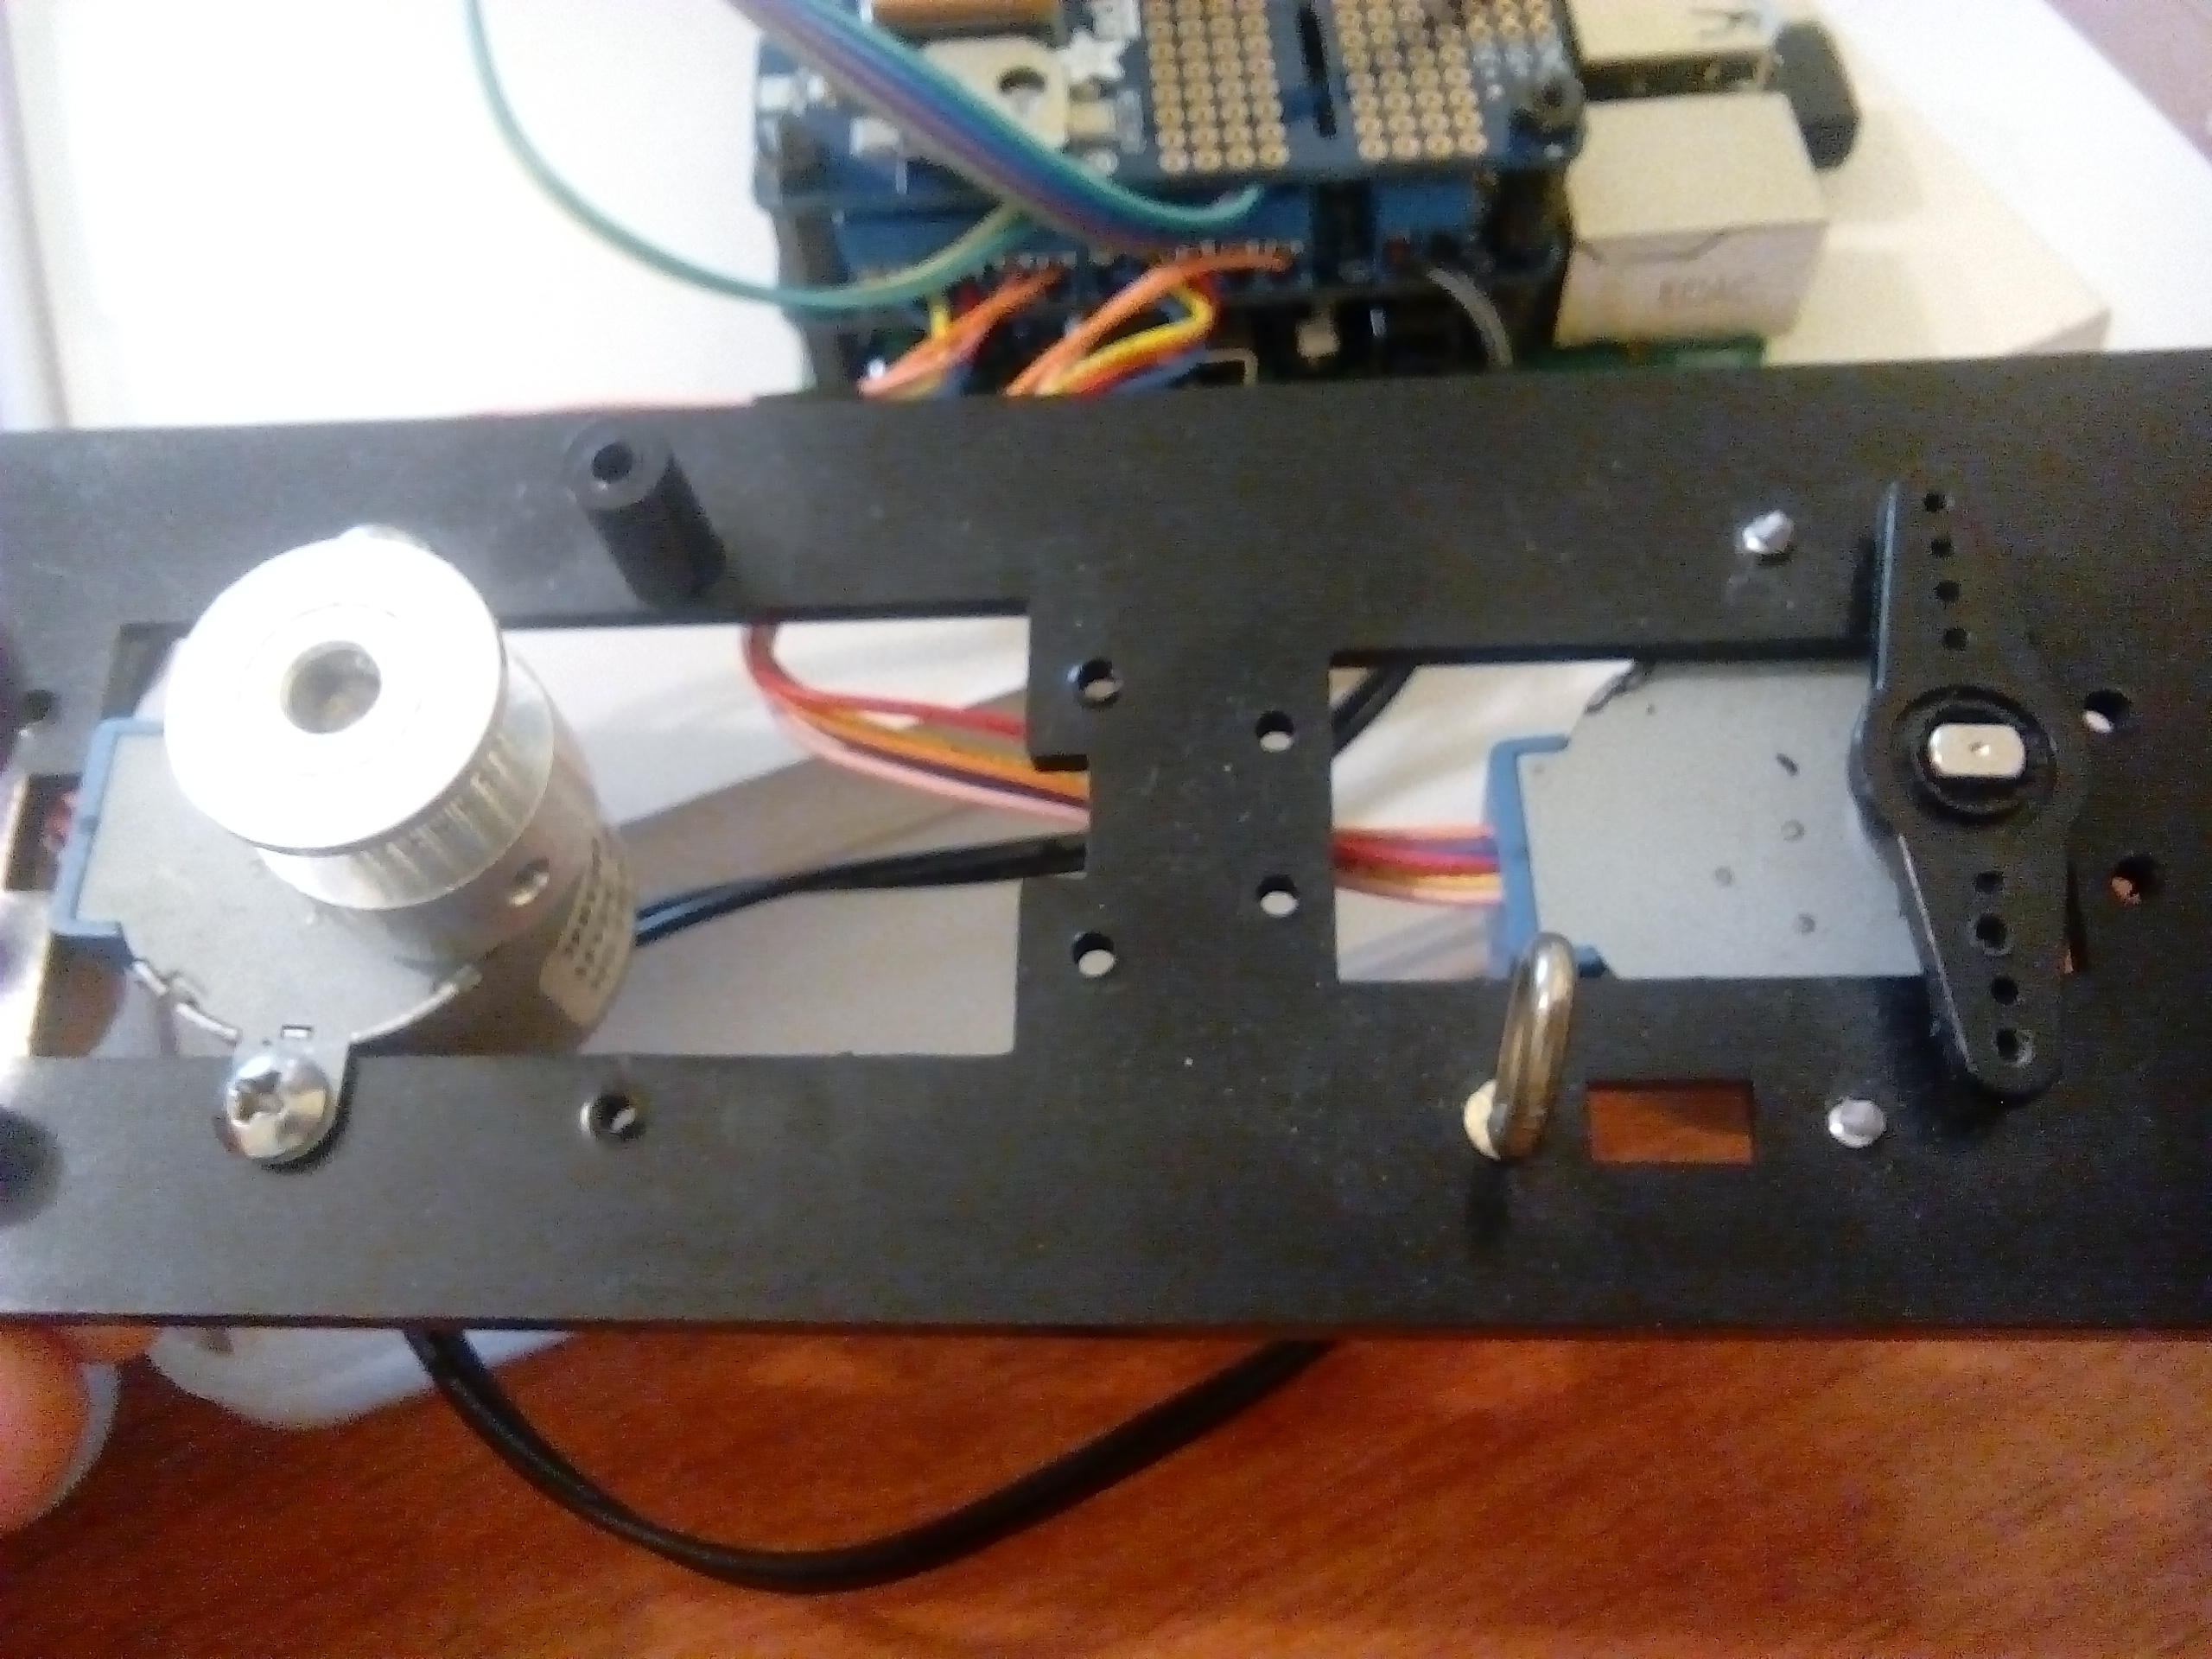
\includegraphics[height=\paperheight,width=\paperwidth]{motors}}
\begin{frame}[plain]
\end{frame}}

\subsection{Motors}
%%%%%%%%%%%%%%%%%%%%%%%%%%%%%%%%%%%%%%%%%%%%%%%%%%%%%%%%%%%%%%%%%%%%
\begin{frame}[fragile]{Motors}
\begin{columns}
\column[t]{0.3\textwidth}
\textbf{Motors software}
\vspace{5mm}
\begin{itemize}
 \item Python - motor hat 
 \item Motor RPIv2 Hat
 \item Stepper Winch (sails)
 \item Servo Rudder
 \end{itemize}
\column[t]{0.7\textwidth}
\begin{center}
 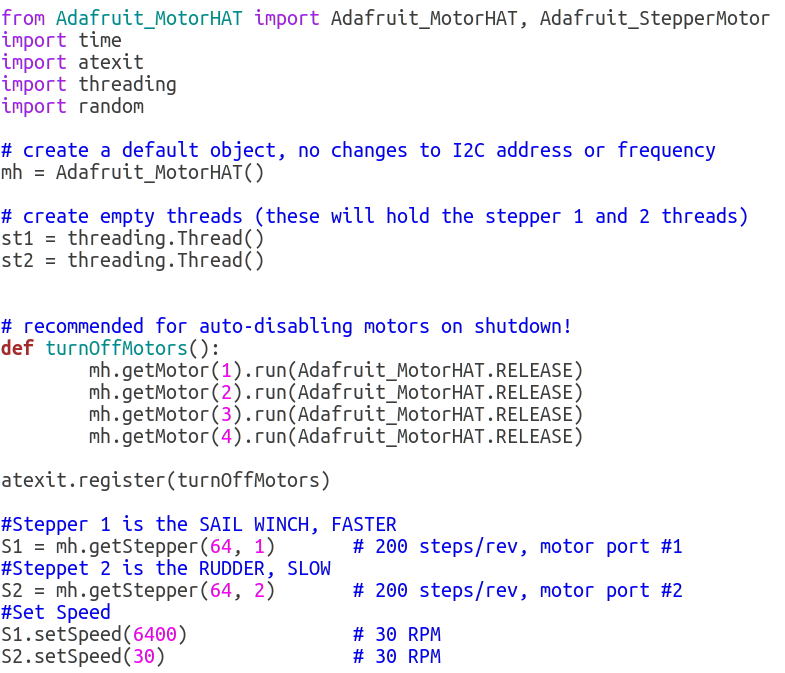
\includegraphics[width=8cm]{motors_py}
\end{center}
\end{columns}
\end{frame}


\subsection{RaspberryPI}
%%%%%%%%%%%%%%%%%%%%%%%%%%%%%%%%%%%%%%%%%%%%%%%%%%%%%%%%%%%%%%%%%%%%
\begin{frame}[fragile]{RaspberryPI}

AmiTomi's brain is the RaspberyPI python code:

\begin{itemize}
 \item Skipper: the captain/navigator software
 \item Waypoint sorter: optimizer for route
 \item Sensor datalogger: simultaneous sensing
 \item Mapper: import data and 3D interpolation 
\end{itemize}
\begin{center}
RaspberryPI GPIO connecting to temperature digital sensors (2m cables)\newline
 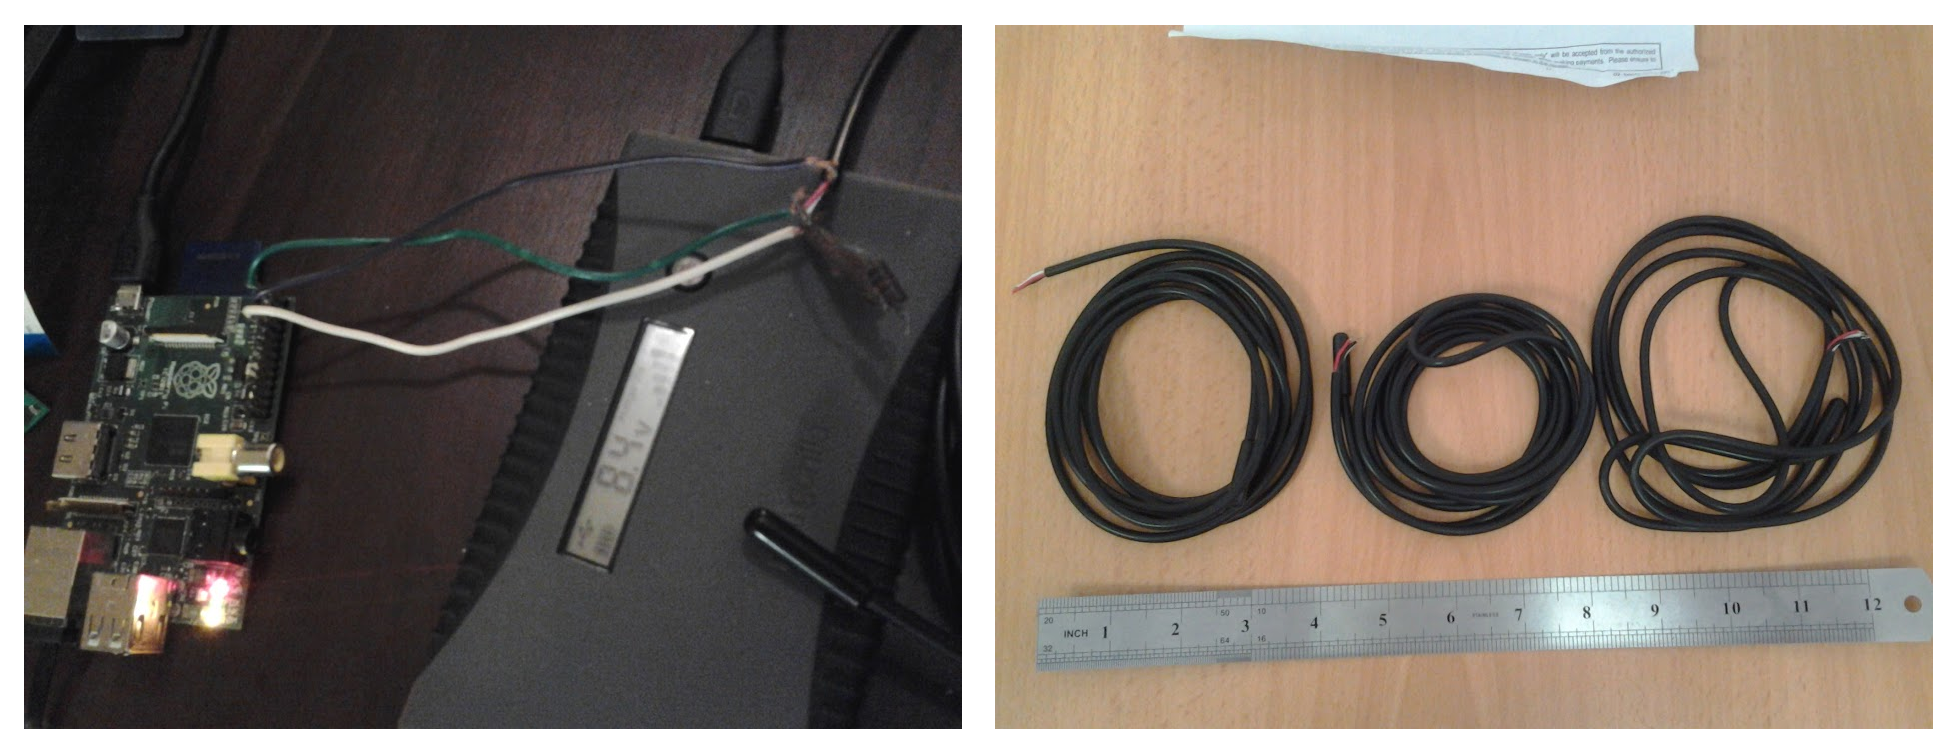
\includegraphics[width=10cm]{temperatureprobes}
\end{center}
\end{frame}

\subsection{Skipper}
%%%%%%%%%%%%%%%%%%%%%%%%%%%%%%%%%%%%%%%%%%%%%%%%%%%%%%%%%%%%%%%%%%%%
\begin{frame}[fragile]{Skipper}
\begin{columns}
\column[t]{0.3\textwidth}
\textbf{Skipper software}
\vspace{5mm}
\begin{itemize}
 \item Python 
 \item Rolls through the whole mission
 \item ``Captain on the Boat''
 \item Use the Waypoints to navigate bearing
 \item Adjust rudder to keep bearing
 \item Adjust sail tension to optimize speed
 \end{itemize}
\column[t]{0.7\textwidth}
\begin{center}
 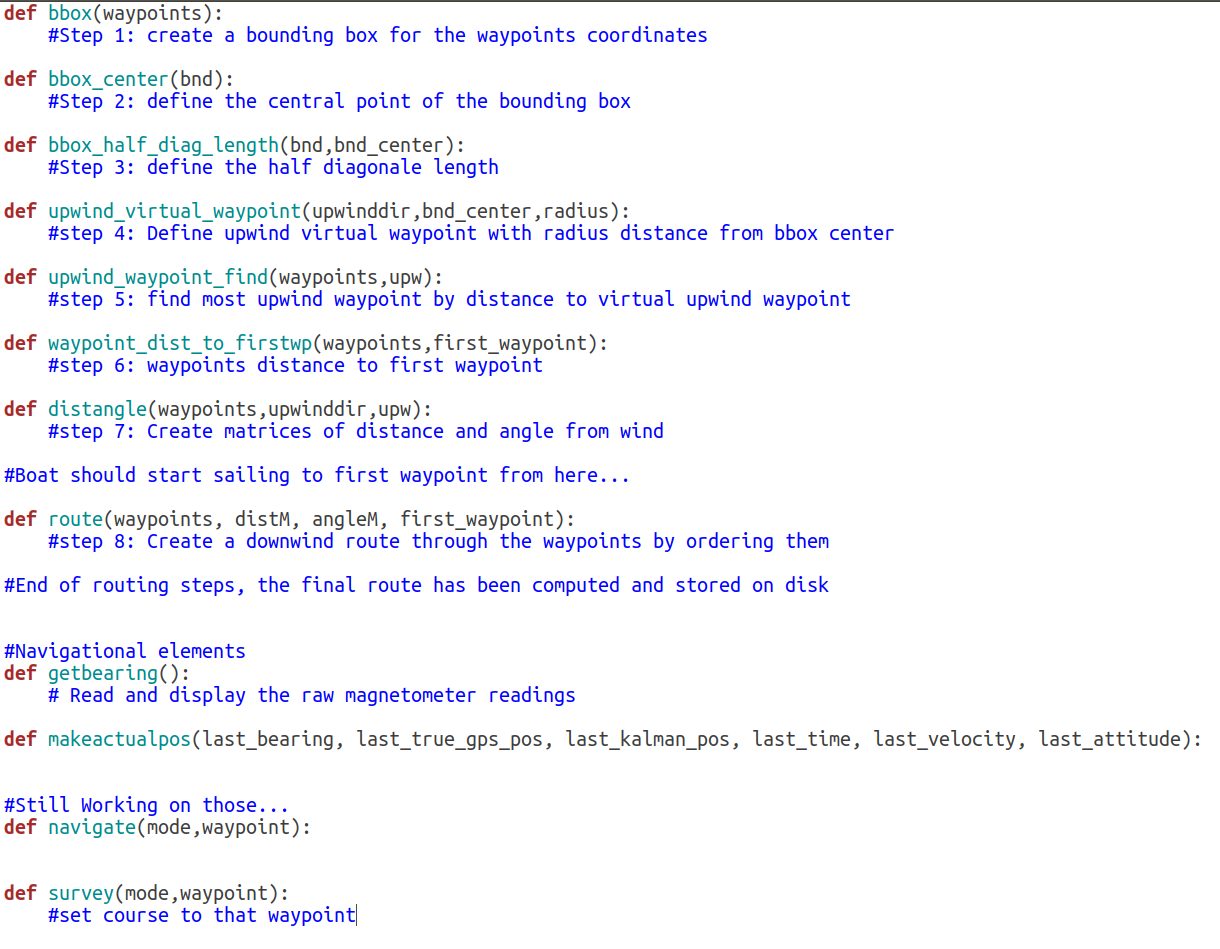
\includegraphics[width=8cm]{skipper_py}
\end{center}
\end{columns}
\end{frame}

\subsection{Waypoints}
%%%%%%%%%%%%%%%%%%%%%%%%%%%%%%%%%%%%%%%%%%%%%%%%%%%%%%%%%%%%%%%%%%%%
\begin{frame}[fragile]{Waypoints}
\begin{columns}
\column[t]{0.4\textwidth}
\textbf{Waypoints sorting software}
\vspace{5mm}
\begin{itemize}
 \item Python-openopt
 \item Assess waypoints
 \item Guess the wind direction
 \item Compute upwind mission start
 \item Compute route through downwind waypoints
 \end{itemize}
\column[t]{0.6\textwidth}
\begin{center}
 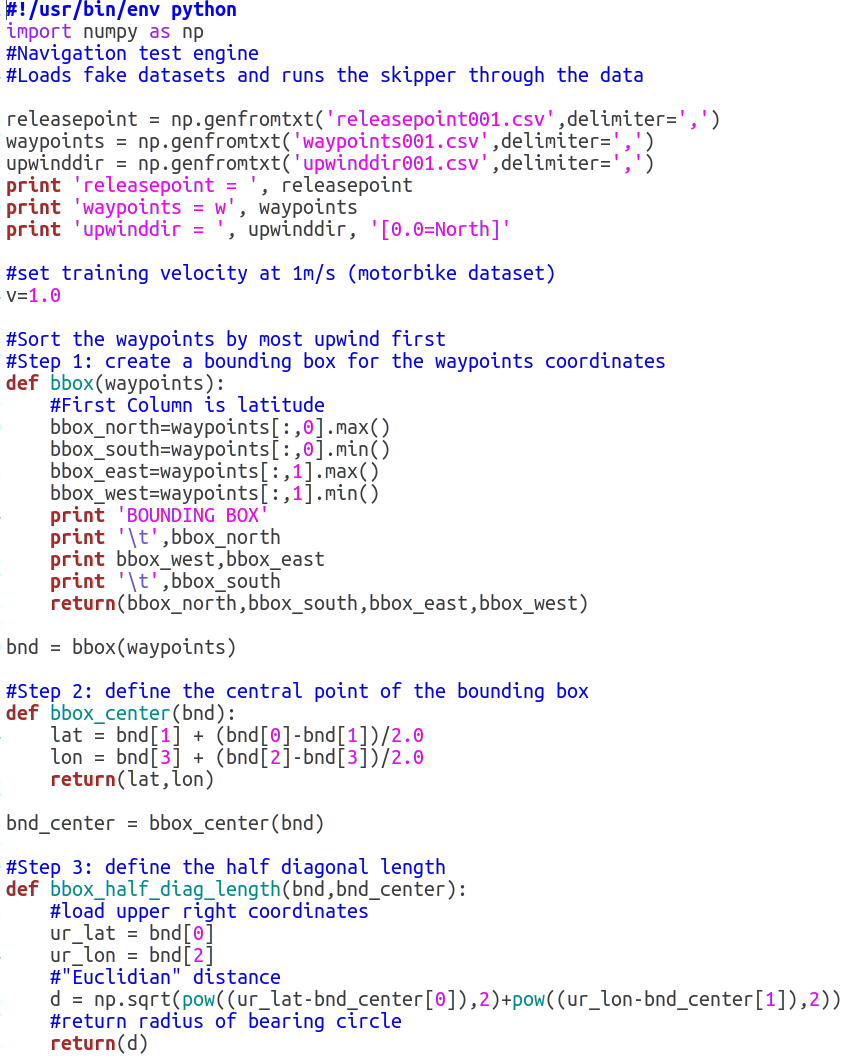
\includegraphics[width=8cm]{waypoints_py}
\end{center}
\end{columns}
\end{frame}


\subsection{Mapping}
%%%%%%%%%%%%%%%%%%%%%%%%%%%%%%%%%%%%%%%%%%%%%%%%%%%%%%%%%%%%%%%%%%%%
\begin{frame}[fragile]{Mapping}
\begin{columns}
\column[t]{0.5\textwidth}
\textbf{Mapping software}
\vspace{5mm}
\begin{itemize}
 \item Python-OGR (GDAL)
 \item pyGRASS
 \item Receive 3 temperature data with Location
 \item Convert to vector data
 \item Compute 3 interpolation layers (in water, on water, in air)
 \item Compute conduction and convection flux
 \item Model evaporation maps
 \end{itemize}
\column[t]{0.5\textwidth}
\begin{center}
 \includegraphics[width=2.75cm]{GDALLogoColor}\\
 
\includegraphics[width=2.75cm]{Grass_GIS}
\end{center}
\end{columns}
\end{frame}


\subsection{FOSS4G}
%%%%%%%%%%%%%%%%%%%%%%%%%%%%%%%%%%%%%%%%%%%%%%%%%%%%%%%%%%%%%%%%%%%%
\begin{frame}[fragile]{FOSS4G software}
\textbf{FOSS and FOSS4G software}\\
\begin{itemize}
 \item Python-gps (GPS data)
 \item Python-i2ctools (Compass/Temperature data)
 \item Python-XloBorg (Compass data)
 \item Python-openopt (Waypoints downwind sorting \href{htp://openopt.org}{openopt.org})
 \item Python-MotorPiTX (servo control for sails \& rudder)
 \item (py)GRASS (live processing of 3D GIS data)
 \item If online: PyWPS, SOS/network reporting. 
\end{itemize}
\end{frame}


\section{Conclusions}
%%%%%%%%%%%%%%%%%%%%%%%%%%%%%%%%%%%%%%%%%%%%%%%%%%%%%%%%%%%%%%%%%%%%
\begin{frame}[fragile]{Conclusions}

\begin{block}{FOSS4G natural extension is Open Source Hardware}
\begin{itemize}
 \item {\bf RaspberryPI:} Small PC (ARM v8, Linux) 
 \item {\bf Arduino:} Micro-controller
 \item {\bf OpenLog:} Data Logger
 \item {\bf GDAL/OGR:} Flexible sensor raw data manipulation
 \item {\bf GRASS GIS:} Mobile FOSS4G powerhouse
 \item {\bf PyWPS:} Online GRASS GIS processing 
 \item {\bf Together:} Flexible all-in-one sensor-to-map solutions
\end{itemize}
\end{block}

\end{frame}

%%%%%%%%%%%%%%%%%%%%%%%%%%%%%%%%%%%%%%%%%%%%%%%%%%%%%%%%%%%%%%%%%%%%
\begin{frame}[fragile]{Thank You}
\textbf{Thank you}
\begin{center}
 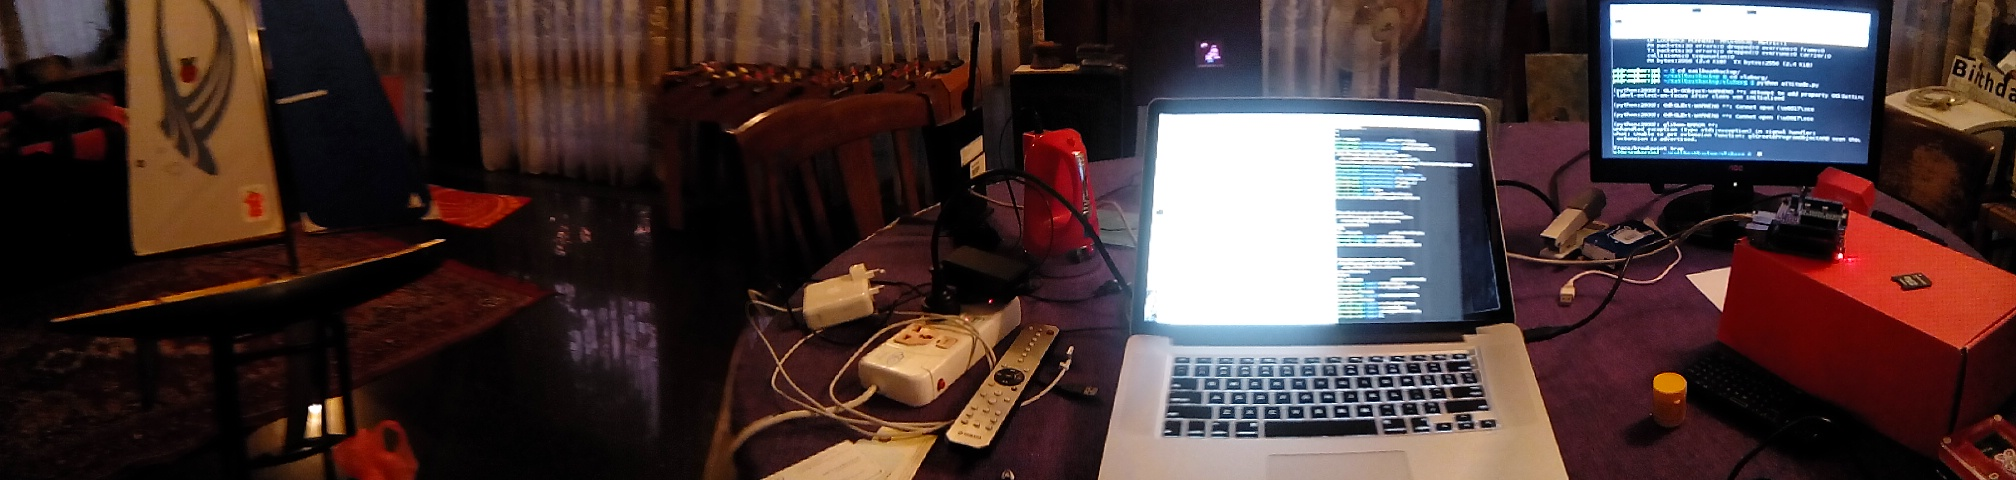
\includegraphics[width=15cm]{pancam}
\end{center}
\end{frame}

\end{document}
